\documentclass[10pt,aspectratio=169]{beamer}

\IfFileExists{/home/torterotot/Documents/PhD-Thesis/README.md}{\def\PhDthesisdir{/home/torterotot/Documents/PhD-Thesis}}{}
\IfFileExists{/home/lucas/Documents/PhD-Thesis/README.md}{\def\PhDthesisdir{/home/lucas/Documents/PhD-Thesis}}{}

\def\PRINTABLE{false}
\IfFileExists{/home/lucas/texmf/tex/latex/ltstyle/ltstyle.sty}{\def\homedir{/home/lucas}}{}
\IfFileExists{/home/torterotot/texmf/tex/latex/ltstyle/ltstyle.sty}{\def\homedir{/home/torterotot}}{}
\RequirePackage[log-declarations=false]{xparse}
\usepackage[english]{babel}
\usepackage[none,Roboto,beamerheader,beamerlogo]{ltstyle}
\usepackage{cmstransversetikz}
% homedir
\ifdefined\homedir \else {%
\IfFileExists{/home/lucas/texmf/tex/latex/ltstyle/ltstyle.sty}{\def\homedir{/home/lucas}}{}%
\IfFileExists{/home/torterotot/texmf/tex/latex/ltstyle/ltstyle.sty}{\def\homedir{/home/torterotot}}{}%
} \fi

% General
\def\NordreNNT{\todo{?}}
\def\LYCEN{\todo{?}}

\def\Hs{\higgs}
\def\Hn{\Higgs}
\def\Ha{\HiggsA}
\def\Hp{\Higgsplus}
\def\Hm{\Higgsminus}
\def\Hu{\Higgsup}
\def\Hd{\Higgsdo}

\newcommand{\higgsSM}{\ensuremath{\higgs_\text{SM}}}
\newcommand{\higgsMSSM}{\ensuremath{\higgs_\text{MSSM}}}
\newcommand{\higgsML}{\ensuremath{\mathcal{H}}}

\newcommand{\SM}{SM}%{modèle standard}

\newcommand {\Lone}{Level-1\xspace} % Level-1 or L1 ?
\newcommand {\Ltwo}{Level-2\xspace}
\newcommand {\Lthree}{Level-3\xspace}

\newcommand{\Lcal}{\ensuremath{\mathcal{L}}}
\newcommand{\LKH}{\ensuremath{\mathfrak{L}}}
\newcommand{\Poisson}{\ensuremath{\mathfrak{P}}}
\newcommand{\Constraint}{\ensuremath{\mathfrak{C}}}
\newcommand{\hypB}{\ensuremath{\mathfrak{b}}}
\newcommand{\hypSB}{\ensuremath{\mathfrak{sb}}}
\newcommand{\hypS}{\ensuremath{\mathfrak{s}}}
\newcommand{\hypH}{\ensuremath{\mathfrak{h}}}
\newcommand{\CLB}{\ensuremath{CL_{\hypB}}}
\newcommand{\CLSB}{\ensuremath{CL_{\hypSB}}}
\newcommand{\CLS}{\ensuremath{CL_{\hypS}}}

\newcommand{\POG}{\emph{POG}}
\newcommand{\PAG}{\emph{PAG}}

\def\DeepCSV{\textsc{DeepCSV}}

\newcommand{\SVFIT}{\textsc{SVfit}}

\def\BR{\ensuremath{\mathcal{BR}}}

\newcommand{\HLTpath}{chemin de déclenchement}
\newcommand{\HLTpaths}{chemins de déclenchement}
\newcommand{\HLTPATH}{Chemin de déclenchement}
\newcommand{\HLTPATHS}{Chemins de déclenchement}

\newcommand{\fakefactor}{facteur de faux}
\newcommand{\fakefactors}{facteurs de faux}
\newcommand{\Fakefactor}{Facteur de faux}
\newcommand{\Fakefactors}{Facteurs de faux}

\newcommand{\refChMSSM}{\ifref{chapter-MS-MSSM}{\ref{chapter-MS-MSSM}}{1}}
\newcommand{\refChLHCCMS}{\ifref{chapter-LHC}{\ref{chapter-LHC}}{2}}
\newcommand{\refChJERC}{\ifref{chapter-JERC}{\ref{chapter-JERC}}{3}}
\newcommand{\refChHTT}{\ifref{chapter-HTT_analysis}{\ref{chapter-HTT_analysis}}{4}}
\newcommand{\refChML}{\ifref{chapter-ML}{\ref{chapter-ML}}{5}}

\newcommand{\refApUNSI}{\ifref{annexe-SI_UN}{\ref{annexe-SI_UN}}{A}}
\newcommand{\refApMath}{\ifref{annexe-maths}{\ref{annexe-maths}}{B}}
\newcommand{\refApFmf}{\ifref{annexe-fmf}{\ref{annexe-fmf}}{C}}
\newcommand{\refApJERCdatasets}{\ifref{annexe-datasets-GJets}{\ref{annexe-datasets-GJets}}{D}}
\newcommand{\refApHTTdatasets}{\ifref{annexe-datasets-HTT}{\ref{annexe-datasets-HTT}}{E}}
\newcommand{\refApHTTtrg}{\ifref{annexe-triggers-HTT}{\ref{annexe-triggers-HTT}}{F}}
\newcommand{\refApHTTctrlplots}{\ifref{annexe-control_plots-HTT}{\ref{annexe-control_plots-HTT}}{G}}
\newcommand{\refApHTTshapes}{\ifref{annexe-discriminating_variables-HTT}{\ref{annexe-discriminating_variables-HTT}}{H}}

% Parties du détecteur
\newcommand{\CMSBarrel}{\emph{Barrel}}
\newcommand{\CMSEndcap}{\emph{Endcap}}
\newcommand{\CMSForward}{\emph{Forward}}

\newcommand{\CMSbarrel}{\emph{barrel}}
\newcommand{\CMSendcap}{\emph{endcap}}
\newcommand{\CMSforward}{\emph{forward}}

\newcommand{\CMSBarrels}{\emph{Barrels}}
\newcommand{\CMSEndcaps}{\emph{Endcaps}}
\newcommand{\CMSForwards}{\emph{Forwards}}

\newcommand{\CMSbarrels}{\emph{barrels}}
\newcommand{\CMSendcaps}{\emph{endcaps}}
\newcommand{\CMSforwards}{\emph{forwards}}

\renewcommand{\CMSBarrel}{Tonneau}
\renewcommand{\CMSEndcap}{Bouchon}
\renewcommand{\CMSForward}{Vers l'avant}

\renewcommand{\CMSbarrel}{tonneau}
\renewcommand{\CMSendcap}{bouchon}
\renewcommand{\CMSforward}{vers l'avant}

\renewcommand{\CMSBarrels}{Tonneaux}
\renewcommand{\CMSEndcaps}{Bouchons}
\renewcommand{\CMSForwards}{\CMSForward}

\renewcommand{\CMSbarrels}{tonneaux}
\renewcommand{\CMSendcaps}{bouchons}
\renewcommand{\CMSforwards}{\CMSforward}

% HTT
\newcommand{\DEEPTAU}{\textsc{DeepTau}}
\newcommand{\ttbar}{\quarkt\antiquarkt}
\newcommand{\Wjet}{\ensuremath{\Wboson+\text{jet}}}
\newcommand{\Wjets}{\ensuremath{\Wboson+\text{jets}}}
\newcommand{\mT}{\ensuremath{m_{\mathrm{T}}}}
\newcommand{\mTtot}{\ensuremath{\mT^{\mathrm{tot}}}}
\newcommand{\msv}{\ensuremath{m_{\SVFIT}}}
\newcommand{\mlmass}{\ensuremath{m_{\mathrm{ML}}}}
\newcommand{\mml}{\mlmass}
\newcommand{\mtt}{\ensuremath{m^{(\tau\tau)}}}
\newcommand{\mvis}{\mtt}
\newcommand{\pTvis}{\ensuremath{\pT^{(\tau\tau)}}}
\newcommand{\vpTvis}{\ensuremath{\vpT^{(\tau\tau)}}}
\newcommand{\Dzeta}{\ensuremath{D_\zeta}}
\newcommand{\minv}{\ensuremath{m_{\mathrm{inv}}}}
\newcommand{\muonID}{\emph{muonID}}
\newcommand{\Njets}{\ensuremath{N_{\textrm{jets}}}}
\newcommand{\Nbjets}{\ensuremath{N_{\textrm{\quarkb-jets}}}}
\newcommand{\Nprebjets}{\ensuremath{N_{\textrm{pre \quarkb-jets}}}}
\newcommand{\mjj}{\ensuremath{m_{\mathrm{jj}}}}
\newcommand{\Detajj}{\ensuremath{\Delta \eta_{\mathrm{jj}}}}
\newcommand{\Ndof}{\ensuremath{N_{\textrm{dof}}}}
\newcommand{\Nmdhits}{\ensuremath{N^{\textrm{MD}}_{\textrm{hits}}}}
\newcommand{\Nms}{\ensuremath{N_{\textrm{MS}}}}
\newcommand{\Npixelhits}{\ensuremath{N^{\textrm{pixel}}_{\textrm{hits}}}}
\newcommand{\Ntrkhits}{\ensuremath{N^{\textrm{tracker}}_{\textrm{hits}}}}
\newcommand{\EleIDMVA}{\emph{electron ID MVA}}
\newcommand{\CutBasedEleID}{\emph{cut-based ID}}
\newcommand{\CutBasedEleIDVeto}{\emph{cut-based veto ID}}
\newcommand{\Nbtag}{\Nbjets}
\newcommand{\mCutForCategories}{\msv}
\newcommand{\mCutForCategoriesdef}{\mCutForCategories\ est la masse du dilepton estimée par \SVFIT~\cite{SVFit_Bianchini_2014}}

\newcommand{\ftauh}{\text{faux~\tauh}}
\newcommand{\ftauhs}{\text{faux~\tauh}}

\newcommand{\FF}{\ensuremath{\mathrm{FF}}}

\newcommand{\GetChannelStr}[1]{%
\ifthenelse{\equal{#1}{tt}}{\tauh\tauh}{}%
\ifthenelse{\equal{#1}{mt}}{\mu\tauh}{}%
\ifthenelse{\equal{#1}{et}}{\ele\tauh}{}%
\ifthenelse{\equal{#1}{mm}}{\mu\mu}{}%
\ifthenelse{\equal{#1}{em}}{\ele\mu}{}%
\ifthenelse{\equal{#1}{ee}}{\ele\ele}{}%
\ifthenelse{\equal{#1}{lt}}{$\ell\tauh$}{}%
\ifthenelse{\equal{#1}{ll}}{$\ell\ell$}{}%
}

\newcommand{\CATnobtag}{\texttt{no-btag}}
\newcommand{\CATbtag}{\texttt{btag}}
\newcommand{\CATlowdz}{\texttt{low-}\Dzeta}
\newcommand{\CATmediumdz}{\texttt{medium-}\Dzeta}
\newcommand{\CAThighdz}{\texttt{high-}\Dzeta}
\newcommand{\CATtightmt}{\texttt{tight-}\mT}
\newcommand{\CATloosemt}{\texttt{loose-}\mT}

\newcommand{\NNscore}{\ensuremath{\mathrm{NN}_{\mathrm{score}}}}

\newcommand{\CATxxh}{\texttt{xxh}}
\newcommand{\CATemb}{\texttt{emb}}
\newcommand{\CATzll}{\texttt{zll}}
\newcommand{\CATttbar}{\texttt{ttbar}}
\newcommand{\CATdib}{\texttt{diboson}}
\newcommand{\CATfake}{\texttt{fake}}
\newcommand{\CATqcd}{\texttt{qcd}}
\newcommand{\CATmisc}{\texttt{misc}}

\newcommand{\CATttbarctrl}{CR \ttbar}

\newcommand{\CATbsm}{\texttt{BSM}}
\newcommand{\CATsm}{\texttt{SM}}

\newcommand{\HLTDoubleTau}{\og double \tauh \fg}
\newcommand{\HLTDoubleMu}{\og double muon \fg}
\newcommand{\HLTSingleTau}{\og \tauh\ seul \fg}
\newcommand{\HLTSingleMu}{\og muon seul \fg}
\newcommand{\HLTMuTauCross}{\og muon et \tauh \fg}
\newcommand{\HLTSingleEle}{\og électron seul \fg}
\newcommand{\HLTEleTauCross}{\og électron et \tauh \fg}

\newcommand{\nfpCLlimit}{\CLS\ à \SI{95}{\%}}
\newcommand{\nfpCLlimitON}{\nfpCLlimit\ sur}

\newcommand{\Neventsaxis}{Événements}
\newcommand{\InclusiveSTR}{inclusif}

\newcommand{\RatiosaxisA}{Rapport au}
\newcommand{\RatiosaxisB}{bruit de fond}

\newcommand{\HTTplotsdir}{HTT_v2}

\newcommand{\GETplotHTTModelIndepLimitsINFOS}[5][\HTTplotsdir]{%

\def\localyaxislabelXXH{\todo{?}}
\ifthenelse{\equal{#4}{ggH}}{
  \def\localyaxislabelXXH{\ensuremath{\gluon\gluon\Phi}}
}{}
\ifthenelse{\equal{#4}{bbH}}{
  \def\localyaxislabelXXH{\ensuremath{\quarkb\antiquarkb\Phi}}
}{}

\def\localxaxislabel{$m_\Phi$ (\SI{}{\GeV})}
\def\localyaxislabel{\nfpCLlimitON\ $\sigma(\localyaxislabelXXH) \times \BR(\Phi\to\tau\tau)$ (\SI{}{\pico\barn})}

% year
\def\locallumivalue{137}\def\localera{Run II}
\ifthenelse{\equal{#3}{2016}}{\def\locallumivalue{35.9}\def\localera{2016}}{}
\ifthenelse{\equal{#3}{2017}}{\def\locallumivalue{41.5}\def\localera{2017}}{}
\ifthenelse{\equal{#3}{2018}}{\def\locallumivalue{59.7}\def\localera{2018}}{}

}

\newcommand{\plotHTTModelIndepLimits}[5][\HTTplotsdir]{%
\begin{tikzpicture}%
\begin{scope}
\clip (.7,.55) -- (.7,7.3) -- (1.25,7.3) -- (1.25,7.11) -- (7.6,7.11) -- (7.6,.55) -- cycle ;
\node[anchor=south west,inner sep=0] at (0,0) {\includegraphics[width=7.85cm]{\PhDthesisdir/plots_and_images/my_plots/#1/limits/#2/mssm_model-independent_#3_#4#5.pdf}};
\fill [white] (1.5, 6) rectangle (3.6, 7);
\end{scope}

\GETplotHTTModelIndepLimitsINFOS[#1]{#2}{#3}{#4}{#5}

\draw (7.7, 0) node [above left] {\footnotesize \localxaxislabel\vphantom{Àq,}};
\draw (0, 7.2) node [below left, rotate=90] {\footnotesize \localyaxislabel\vphantom{Àq,}};
\draw (7.7, 7) node [above left] {\scriptsize \SI{\locallumivalue}{\femto\barn^{-1}} (\localera, \SI{13}{\TeV})\vphantom{Àq,}};

% CMS disclaimer
\draw (1.15, 7) node [above right] {\scriptsize CMS Data\vphantom{Àq,}};
\draw (2.35, 6.75) node [below, text width=1cm] {\centering\scriptsize \WorkInProgress\par};
\end{tikzpicture}%
}

\newcommand{\GETplotHTTModelDepLimitsINFOS}[3][\HTTplotsdir]{%

\def\localxaxislabelptc{\HiggsA}
\ifthenelse{\equal{#2}{mssm_vs_sm_CPV}\or\equal{#2}{mssm_vs_sm_CPV-new_categories}}{
  \def\localxaxislabelptc{\Higgspm}
}{}

\def\localxaxislabel{$m_{\localxaxislabelptc}$ (\SI{}{\GeV})}
\def\localyaxislabel{$\tan\beta$}

}

\newcommand{\plotHTTModelDepLimits}[3][\HTTplotsdir]{%
\begin{tikzpicture}%
\begin{scope}
\clip (.5,.55) -- (.5,7.11) -- (7.675,7.11) -- (7.675,.55) -- cycle ;
\node[anchor=south west,inner sep=0] at (0,0) {\includegraphics[width=7.85cm]{\PhDthesisdir/plots_and_images/my_plots/#1/limits/#2/mssm_mh125_#2#3.pdf}};
\end{scope}

\GETplotHTTModelDepLimitsINFOS[#1]{#2}{#3}

\draw (7.5, 0) node [above left] {\footnotesize \localxaxislabel\vphantom{Àq,}};
\draw (0, 6.2) node [below left, rotate=90] {\footnotesize \localyaxislabel\vphantom{Àq,}};

% year
\draw (7.55, 7) node [above left] {\scriptsize \SI{137}{\femto\barn^{-1}} (Run II, \SI{13}{\TeV})\vphantom{Àq,}};

% CMS disclaimer
\draw (.8, 7) node [above right] {\scriptsize CMS Data\vphantom{Àq,}};
\draw (2.35, 7) node [below, text width=1cm] {\centering\scriptsize \WorkInProgress\par};
\end{tikzpicture}%
}

\newcommand{\GETplotHTTcontrolINFO}[5][\HTTplotsdir]{%

% cuts
\def\localcat{\InclusiveSTR{}}
\ifthenelse{\equal{#3}{emb_ff_high_ml_mass}}{\def\localcat{$\mml>\SI{250}{\GeV}$}}{}
\ifthenelse{\equal{#3}{emb_ff_high_m_sv_puppi}}{\def\localcat{$\msv>\SI{250}{\GeV}$}}{}

% channel
\ifthenelse{\equal{#4}{tt}}{\def\localchannel{\tauh\tauh}\def\localLA{\ensuremath{\tauh^{(1)}}}\def\localLB{\ensuremath{\tauh^{(2)}}}}{}
\ifthenelse{\equal{#4}{mt}}{\def\localchannel{\mu\tauh}\def\localLA{\mu}\def\localLB{\ensuremath{\tauh}}}{}
\ifthenelse{\equal{#4}{et}}{\def\localchannel{\ele\tauh}\def\localLA{\ele}\def\localLB{\ensuremath{\tauh}}}{}
\ifthenelse{\equal{#4}{em}}{\def\localchannel{\ele\mu}\def\localLA{\ele}\def\localLB{\mu}}{}

% year
\ifthenelse{\equal{#2}{2016}}{\def\locallumivalue{35.9}}{}
\ifthenelse{\equal{#2}{2017}}{\def\locallumivalue{41.5}}{}
\ifthenelse{\equal{#2}{2018}}{\def\locallumivalue{59.7}}{}

% axis labels
\def\localxaxislabel{\todo{\inlinecode{bash}{#5}}}
\def\localyaxislabel{\todo{Y?}}
\ifthenelse{\equal{#5}{bpt_1}}{
  \def\localxaxislabel{$\pT (\text{\quarkb-jet principal})$ (\SI{}{\GeV})}
  \def\localyaxislabel{$\dd{\,\text{\Neventsaxis}}/\dd{\pT}$ (\SI{}{\GeV^{-1}})}
}{}
\ifthenelse{\equal{#5}{bpt_2}}{
  \def\localxaxislabel{$\pT (\text{\quarkb-jet secondaire})$ (\SI{}{\GeV})}
  \def\localyaxislabel{$\dd{\,\text{\Neventsaxis}}/\dd{\pT}$ (\SI{}{\GeV^{-1}})}
}{}
\ifthenelse{\equal{#5}{jpt_1}}{
  \def\localxaxislabel{$\pT (\text{jet principal})$ (\SI{}{\GeV})}
  \def\localyaxislabel{$\dd{\,\text{\Neventsaxis}}/\dd{\pT}$ (\SI{}{\GeV^{-1}})}
}{}
\ifthenelse{\equal{#5}{jpt_2}}{
  \def\localxaxislabel{$\pT (\text{jet secondaire})$ (\SI{}{\GeV})}
  \def\localyaxislabel{$\dd{\,\text{\Neventsaxis}}/\dd{\pT}$ (\SI{}{\GeV^{-1}})}
}{}
\ifthenelse{\equal{#5}{jpt_r}}{
  \def\localxaxislabel{$\pT (\text{activité hadronique additionnelle})$ (\SI{}{\GeV})}
  \def\localyaxislabel{$\dd{\,\text{\Neventsaxis}}/\dd{\pT}$ (\SI{}{\GeV^{-1}})}
}{}
\ifthenelse{\equal{#5}{jeta_1}}{
  \def\localxaxislabel{$\eta (\text{jet principal})$}
  \def\localyaxislabel{$\dd{\,\text{\Neventsaxis}}/\dd{\eta}$}
}{}
\ifthenelse{\equal{#5}{jeta_2}}{
  \def\localxaxislabel{$\eta (\text{jet secondaire})$}
  \def\localyaxislabel{$\dd{\,\text{\Neventsaxis}}/\dd{\eta}$}
}{}
\ifthenelse{\equal{#5}{jeta_r}}{
  \def\localxaxislabel{$\eta (\text{activité hadronique additionnelle})$}
  \def\localyaxislabel{$\dd{\,\text{\Neventsaxis}}/\dd{\eta}$}
}{}
\ifthenelse{\equal{#5}{jphi_1}}{
  \def\localxaxislabel{$\phi (\text{jet principal})$}
  \def\localyaxislabel{$\dd{\,\text{\Neventsaxis}}/\dd{\phi}$}
}{}
\ifthenelse{\equal{#5}{jphi_2}}{
  \def\localxaxislabel{$\phi (\text{jet secondaire})$}
  \def\localyaxislabel{$\dd{\,\text{\Neventsaxis}}/\dd{\phi}$}
}{}
\ifthenelse{\equal{#5}{jphi_r}}{
  \def\localxaxislabel{$\phi (\text{activité hadronique additionnelle})$}
  \def\localyaxislabel{$\dd{\,\text{\Neventsaxis}}/\dd{\phi}$}
}{}
\ifthenelse{\equal{#5}{nbtag}}{
  \def\localxaxislabel{\Nbjets}
  \def\localyaxislabel{\Neventsaxis}
}{}
\ifthenelse{\equal{#5}{njets}}{
  \def\localxaxislabel{\Njets}
  \def\localyaxislabel{\Neventsaxis}
}{}
\ifthenelse{\equal{#5}{Njet_r}}{
  \def\localxaxislabel{\Njetsr}
  \def\localyaxislabel{\Neventsaxis}
}{}
\ifthenelse{\equal{#5}{npv}}{
  \def\localxaxislabel{\Npu}
  \def\localyaxislabel{\Neventsaxis}
}{}
\ifthenelse{\equal{#5}{dijetpt}}{
  \def\localxaxislabel{$\pT (\text{2 jets principaux})$ (\SI{}{\GeV})}
  \def\localyaxislabel{$\dd{\,\text{\Neventsaxis}}/\dd{\pT}$ (\SI{}{\GeV^{-1}})}
}{}
\ifthenelse{\equal{#5}{jdeta}}{
  \def\localxaxislabel{$\Detajj (\text{2 jets principaux})$}
  \def\localyaxislabel{$\dd{\,\text{\Neventsaxis}}/\dd{\Detajj}$}
}{}
\ifthenelse{\equal{#5}{mjj}}{
  \def\localxaxislabel{$\mjj (\text{2 jets principaux})$ (\SI{}{\GeV})}
  \def\localyaxislabel{$\dd{\,\text{\Neventsaxis}}/\dd{m}$ (\SI{}{\GeV^{-1}})}
}{}
\ifthenelse{\equal{#5}{pt_1}}{
  \def\localxaxislabel{$\pT(\localLA)$ (\SI{}{\GeV})}
  \def\localyaxislabel{$\dd{\,\text{\Neventsaxis}}/\dd{\pT}$ (\SI{}{\GeV^{-1}})}
}{}
\ifthenelse{\equal{#5}{pt_2}}{
  \def\localxaxislabel{$\pT(\localLB)$ (\SI{}{\GeV})}
  \def\localyaxislabel{$\dd{\,\text{\Neventsaxis}}/\dd{\pT}$ (\SI{}{\GeV^{-1}})}
}{}
\ifthenelse{\equal{#5}{eta_1}}{
  \def\localxaxislabel{$\eta (\localLA)$}
  \def\localyaxislabel{$\dd{\,\text{\Neventsaxis}}/\dd{\eta}$}
}{}
\ifthenelse{\equal{#5}{eta_2}}{
  \def\localxaxislabel{$\eta (\localLB)$}
  \def\localyaxislabel{$\dd{\,\text{\Neventsaxis}}/\dd{\eta}$}
}{}
\ifthenelse{\equal{#5}{phi_1}}{
  \def\localxaxislabel{$\phi (\localLA)$}
  \def\localyaxislabel{$\dd{\,\text{\Neventsaxis}}/\dd{\phi}$}
}{}
\ifthenelse{\equal{#5}{phi_2}}{
  \def\localxaxislabel{$\phi (\localLB)$}
  \def\localyaxislabel{$\dd{\,\text{\Neventsaxis}}/\dd{\phi}$}
}{}
\ifthenelse{\equal{#5}{mt_1_puppi}}{
  \def\localxaxislabel{$\mT(\localLA,\MET)$ (\SI{}{\GeV})}
  \def\localyaxislabel{$\dd{\,\text{\Neventsaxis}}/\dd{\mT}$ (\SI{}{\GeV^{-1}})}
}{}
\ifthenelse{\equal{#5}{mt_2_puppi}}{
  \def\localxaxislabel{$\mT(\localLB,\MET)$ (\SI{}{\GeV})}
  \def\localyaxislabel{$\dd{\,\text{\Neventsaxis}}/\dd{\mT}$ (\SI{}{\GeV^{-1}})}
}{}
\ifthenelse{\equal{#5}{mTdileptonMET_puppi}}{
  \def\localxaxislabel{$\mT(\localLA+\localLB,\MET)$ (\SI{}{\GeV})}
  \def\localyaxislabel{$\dd{\,\text{\Neventsaxis}}/\dd{\mT}$ (\SI{}{\GeV^{-1}})}
}{}
\ifthenelse{\equal{#5}{pZetaPuppiMissVis}}{
  \def\localxaxislabel{$\Dzeta$ (\SI{}{\GeV})}
  \def\localyaxislabel{$\dd{\,\text{\Neventsaxis}}/\dd{\Dzeta}$ (\SI{}{\GeV^{-1}})}
}{}
\ifthenelse{\equal{#5}{pt_tt_puppi}}{
  \def\localxaxislabel{$\pT (\localLA+\localLB+\MET)$ (\SI{}{\GeV})}
  \def\localyaxislabel{$\dd{\,\text{\Neventsaxis}}/\dd{\pT}$ (\SI{}{\GeV^{-1}})}
}{}
\ifthenelse{\equal{#5}{DiTauDeltaR}}{
  \def\localxaxislabel{$\Delta R (\localLA,\localLB)$}
  \def\localyaxislabel{$\dd{\,\text{\Neventsaxis}}/\dd{\Delta R}$}
}{}
\ifthenelse{\equal{#5}{m_sv_puppi}}{
  \def\localxaxislabel{$\msv$ (\SI{}{\GeV})}
  \def\localyaxislabel{$\dd{\,\text{\Neventsaxis}}/\dd{m}$ (\SI{}{\GeV^{-1}})}
}{}
\ifthenelse{\equal{#5}{puppimet}}{
  \def\localxaxislabel{$\MET$ (\SI{}{\GeV})}
  \def\localyaxislabel{$\dd{\,\text{\Neventsaxis}}/\dd{\MET}$ (\SI{}{\GeV^{-1}})}
}{}
\ifthenelse{\equal{#5}{puppimetphi}}{
  \def\localxaxislabel{$\phi(\MET)$}
  \def\localyaxislabel{$\dd{\,\text{\Neventsaxis}}/\dd{\phi}$}
}{}
\ifthenelse{\equal{#5}{m_vis}}{
  \def\localxaxislabel{$\mvis$ (\SI{}{\GeV})}
  \def\localyaxislabel{$\dd{\,\text{\Neventsaxis}}/\dd{m}$ (\SI{}{\GeV^{-1}})}
}{}
\ifthenelse{\equal{#5}{ptvis}}{
  \def\localxaxislabel{$\pTvis$ (\SI{}{\GeV})}
  \def\localyaxislabel{$\dd{\,\text{\Neventsaxis}}/\dd{\pT}$ (\SI{}{\GeV^{-1}})}
}{}
\ifthenelse{\equal{#5}{ml_mass}}{
  \def\localxaxislabel{$\mlmass$ (\SI{}{\GeV})}
  \def\localyaxislabel{$\dd{\,\text{\Neventsaxis}}/\dd{m}$ (\SI{}{\GeV^{-1}})}
}{}
\ifthenelse{\equal{#5}{mt_tot_puppi}}{
  \def\localxaxislabel{$\mTtot$ (\SI{}{\GeV})}
  \def\localyaxislabel{$\dd{\,\text{\Neventsaxis}}/\dd{m}$ (\SI{}{\GeV^{-1}})}
}{}

}

\newcommand{\plotHTTcontrol}[5][\HTTplotsdir]{%
\begin{tikzpicture}%
\clip (0,.1) rectangle (7.76,7.7) ;
\begin{scope}
\clip (.45,.55) -- (.45,3) -- (.42,8) -- (1,8) -- (1,7.1) -- (7.76,7.1) -- (7.76,.55) -- cycle ;
\node[anchor=south west,inner sep=0] at (0,0) {\includegraphics[width=7.85cm]{\PhDthesisdir/plots_and_images/my_plots/#1/control_plots/Run#2_plots_#3/#4/Run#2_#4_#5.pdf}};
\end{scope}

\GETplotHTTcontrolINFO[#1]{#2}{#3}{#4}{#5}

% channel & cat
\draw (1, 7) node [above right] {\scriptsize \localchannel, \localcat\vphantom{Àq,}};

% year & lumi
\draw (7.7, 7) node [above left] {\scriptsize \SI{\locallumivalue}{\femto\barn^{-1}} (#2, \SI{13}{\TeV})\vphantom{Àq,}};

% axis labels
\draw (7.7, 0) node [above left] {\footnotesize \localxaxislabel\vphantom{Àq,}};
\draw (-.1, 7.3) node [below left, rotate=90] {\footnotesize \localyaxislabel\vphantom{Àq,}};

\draw (-.1, 1.75) node (tmp) [below, rotate=90] {\scriptsize \RatiosaxisA\vphantom{Àq,}};
\draw (tmp) node [below, rotate=90] {\scriptsize \RatiosaxisB\vphantom{Àq,}};

% CMS disclaimer
\draw (1.85, 7.05) node [below] {\scriptsize CMS Data\vphantom{Àq,}};
\draw (1.85, 6.55) node [below, text width=1cm] {\centering\scriptsize \WorkInProgress\par};
\end{tikzpicture}%
}

\newcommand{\GETplotHTTshapesINFO}[7][\HTTplotsdir]{%

% year
\ifthenelse{\equal{#4}{2016}}{\def\locallumivalue{35.9}}{}
\ifthenelse{\equal{#4}{2017}}{\def\locallumivalue{41.5}}{}
\ifthenelse{\equal{#4}{2018}}{\def\locallumivalue{59.7}}{}

% channel
\ifthenelse{\equal{#5}{tt}}{\def\localchannel{\tauh\tauh}\def\localLA{\ensuremath{\tauh^{(1)}}}\def\localLB{\ensuremath{\tauh^{(2)}}}}{}
\ifthenelse{\equal{#5}{mt}}{\def\localchannel{\mu\tauh}\def\localLA{\mu}\def\localLB{\ensuremath{\tauh}}}{}
\ifthenelse{\equal{#5}{et}}{\def\localchannel{\ele\tauh}\def\localLA{\ele}\def\localLB{\ensuremath{\tauh}}}{}
\ifthenelse{\equal{#5}{em}}{\def\localchannel{\ele\mu}\def\localLA{\ele}\def\localLB{\mu}}{}

% category and variable
\def\localBSMvar{\mTtot}
\ifthenelse{\equal{#2}{m_ml}}{\def\localBSMvar{\mml}}{}
\def\localSMvar{\NNscore}
\def\localSMvarBD{\text{\NNscore\ 2D}}
%\ifthenelse{\equal{#1}{HTT_v1}}{\def\localSMvar{\msv}}{}
\def\localcat{\InclusiveSTR{}}
\def\localvar{\localBSMvar}
\def\localBSM{}
\def\localSM{}
\ifthenelse{\equal{#3}{mssm_vs_sm_h125}}{\def\localBSM{\CATbsm\ }\def\localSM{\CATsm\ }}{}
\def\localSMBSM{}

\ifthenelse{\equal{#6}{1}}{
  \def\localcat{\CATxxh}
  \def\localvar{\localSMvarBD}
}{}
\ifthenelse{\equal{#6}{2}}{
  \def\localcat{\CATttbarctrl}
  \def\localvar{\localBSMvar}
  \def\localSMBSM{\localBSM}
}{}
\ifthenelse{\equal{#6}{13}}{
  \def\localcat{\CATttbar}
  \def\localvar{\localSMvar}
}{}
\ifthenelse{\equal{#6}{14}}{
  \def\localcat{\CATqcd}
  \def\localvar{\localSMvar}
}{}
\ifthenelse{\equal{#6}{15}}{
  \def\localcat{\CATzll}
  \def\localvar{\localSMvar}
}{}
\ifthenelse{\equal{#6}{16}}{
  \def\localcat{\CATmisc}
  \def\localvar{\localSMvar}
}{}
\ifthenelse{\equal{#6}{19}}{
  \def\localcat{\CATdib}
  \def\localvar{\localSMvar}
}{}
\ifthenelse{\equal{#6}{20}}{
  \def\localcat{\CATemb}
  \def\localvar{\localSMvar}
}{}
\ifthenelse{\equal{#6}{21}}{
  \def\localcat{\CATfake}
  \def\localvar{\localSMvar}
}{}
\ifthenelse{\equal{#6}{32}}{
  \def\localcat{\CATnobtag\ \CATtightmt}
    \ifthenelse{\equal{#5}{tt}}{
      \def\localcat{\CATnobtag}
    }{}
    \ifthenelse{\equal{#5}{em}}{
      \def\localcat{\CATnobtag\ \CAThighdz}
    }{}
  \def\localvar{\localBSMvar}
  \def\localSMBSM{\localBSM}
}{}
\ifthenelse{\equal{#6}{33}}{
  \def\localcat{\CATnobtag\ \CATloosemt}
    \ifthenelse{\equal{#5}{em}}{
      \def\localcat{\CATnobtag\ \CATmediumdz}
    }{}
  \def\localvar{\localBSMvar}
  \def\localSMBSM{\localBSM}
}{}
\ifthenelse{\equal{#6}{34}}{
  \def\localcat{\CATnobtag\ \CATlowdz}
  \def\localvar{\localBSMvar}
  \def\localSMBSM{\localBSM}
}{}
\ifthenelse{\equal{#6}{35}}{
  \def\localcat{\CATbtag\ \CATtightmt}
    \ifthenelse{\equal{#5}{tt}}{
      \def\localcat{\CATbtag}
    }{}
    \ifthenelse{\equal{#5}{em}}{
      \def\localcat{\CATbtag\ \CAThighdz}
    }{}
  \def\localvar{\localBSMvar}
  \def\localSMBSM{\localBSM}
}{}
\ifthenelse{\equal{#6}{36}}{
  \def\localcat{\CATbtag\ \CATloosemt}
    \ifthenelse{\equal{#5}{em}}{
      \def\localcat{\CATbtag\ \CATmediumdz}
    }{}
  \def\localvar{\localBSMvar}
  \def\localSMBSM{\localBSM}
}{}
\ifthenelse{\equal{#6}{37}}{
  \def\localcat{\CATbtag\ \CATlowdz}
  \def\localvar{\localBSMvar}
  \def\localSMBSM{\localBSM}
}{}

\ifthenelse{\equal{#3}{cut_based_sm}}{
\def\localSMvar{\msv}
\ifthenelse{\equal{#2}{m_ml}}{\def\localSMvar{\mml}}{}
\def\localBSMvar{\localSMvar}
\def\localvar{\localSMvar}

\def\localcat{\todo{???}}

\def\localBSM{}
\def\localSM{}
\def\localSMBSM{}

\ifthenelse{\equal{#5}{tt}}{
  \ifthenelse{\equal{#6}{10}}{
    \def\localcat{$\Njets=0, \Delta R < \num{3.2}$}
  }{}
  \ifthenelse{\equal{#6}{11}}{
    \def\localcat{$\Njets=1, \num{2.5} \leq \Delta R \!<\! \num{3.2}, \pT(\tau\tau) \!<\! \SI{100}{\GeV}$}
  }{}
  \ifthenelse{\equal{#6}{12}}{
    \def\localcat{$\Njets=1, \Delta R \!<\! \num{2.5}, \pT(\tau\tau) \!<\! \SI{100}{\GeV}$}
  }{}
  \ifthenelse{\equal{#6}{13}}{
    \def\localcat{$\Njets=1, \Delta R \!<\! \num{2.5}, \pT(\tau\tau) \geq \SI{100}{\GeV}$}
  }{}
  \ifthenelse{\equal{#6}{14}}{
    \def\localcat{$\Delta R \!<\! \num{2.5}, \mjj\!>\!\SI{350}{\GeV}, \Detajj\geq4$}
  }{}
  \ifthenelse{\equal{#6}{15}}{
    \def\localcat{$\Delta R \!<\! \num{2.5}, \mjj\!>\!\SI{350}{\GeV}, \Detajj\!<\!4$}
  }{}
  \ifthenelse{\equal{#6}{16}}{
    \def\localcat{$\Delta R \!<\! \num{2.5}, \mjj\!<\!\SI{350}{\GeV}$}
  }{}
  \ifthenelse{\equal{#6}{17}}{
    \def\localcat{$\binom{\Njets\geq2, \Delta R \geq \num{2.5}}{\Njets<2, \Delta R \geq \num{3.2}}$}
  }{}
}{}

\ifthenelse{\equal{#5}{mt}\or\equal{#5}{et}}{
  \ifthenelse{\equal{#6}{10}}{
    \def\localcat{$\Njets=0, \CATtightmt$}
  }{}
  \ifthenelse{\equal{#6}{11}}{
    \def\localcat{$\Njets=0, \CATloosemt$}
  }{}
  \ifthenelse{\equal{#6}{12}}{
    \def\localcat{$\Njets\geq1, \Delta R \geq \num{2.5}$}
  }{}
  \ifthenelse{\equal{#6}{13}}{
    \def\localcat{$\Njets=1, \Delta R \!<\! \num{2.5}, \pT(\tau\tau) \!<\! \SI{120}{\GeV}$}
  }{}
  \ifthenelse{\equal{#6}{14}}{
    \def\localcat{$\Njets=1, \Delta R \!<\! \num{2.5}, \SI{120}{\GeV} \!<\! \pT(\tau\tau) \!<\! \SI{200}{\GeV}$}
  }{}
  \ifthenelse{\equal{#6}{15}}{
    \def\localcat{$\Njets=1, \Delta R \!<\! \num{2.5}, \pT(\tau\tau) \!>\! \SI{200}{\GeV}$}
  }{}
  \ifthenelse{\equal{#6}{16}}{
    \def\localcat{$\Njets\geq2, \Delta R \!<\! \num{2.5}, \mjj \!<\! \SI{350}{\GeV}$}
    \def\localcat{$\Delta R \!<\! \num{2.5}, \mjj \!<\! \SI{350}{\GeV}$}
  }{}
  \ifthenelse{\equal{#6}{17}}{
    \def\localcat{$\Njets\geq2, \Delta R \!<\! \num{2.5}, \SI{350}{\GeV} \!<\! \mjj \!<\! \SI{1}{\TeV}$}
  }{}
  \ifthenelse{\equal{#6}{18}}{
    \def\localcat{$\Njets\geq2, \Delta R \!<\! \num{2.5}, \mjj \!>\! \SI{1}{\TeV}$}
    \def\localcat{$\Delta R \!<\! \num{2.5}, \mjj \!>\! \SI{1}{\TeV}$}
  }{}
}{}

\ifthenelse{\equal{#5}{em}}{
  \ifthenelse{\equal{#6}{10}}{
    \def\localcat{$\Njets=0, -35 \!<\! \Dzeta \!<\! -10, \pT(\tau\tau) \!>\! 10$}
  }{}
  \ifthenelse{\equal{#6}{11}}{
    \def\localcat{$\Njets=0, -35 \!<\! \Dzeta \!<\! -10, \pT(\tau\tau) \!<\! 10$}
  }{}
  \ifthenelse{\equal{#6}{12}}{
    \def\localcat{$\Njets=0, \Dzeta \!>\! -10, \pT(\tau\tau) \!>\! 10$}
  }{}
  \ifthenelse{\equal{#6}{13}}{
    \def\localcat{$\Njets=0, \Dzeta \!>\! -10, \pT(\tau\tau) \!<\! 10$}
  }{}
  \ifthenelse{\equal{#6}{14}}{
    \def\localcat{$\Njets=1, \SI{120} \!<\! \pT(\tau\tau) \!<\! \SI{200}{\GeV}$}
  }{}
  \ifthenelse{\equal{#6}{15}}{
    \def\localcat{$\Njets=1, \SI{40} \!<\! \pT(\tau\tau) \!<\! \SI{120}{\GeV}$}
  }{}
  \ifthenelse{\equal{#6}{16}}{
    \def\localcat{$\Njets=1, \pT(\tau\tau) \!>\! \SI{200}{\GeV}$}
  }{}
  \ifthenelse{\equal{#6}{17}}{
    \def\localcat{$\Njets=1, \pT(\tau\tau) \!<\! \SI{40}{\GeV}$}
  }{}
  \ifthenelse{\equal{#6}{18}}{
    \def\localcat{$\Njets\geq2, \mjj \!>\! \SI{350}{\GeV}$}
  }{}
  \ifthenelse{\equal{#6}{19}}{
    \def\localcat{$\Njets\geq2, \mjj \!<\! \SI{350}{\GeV}$}
  }{}
}{}

}{}

% axis labels
\def\localxaxislabel{\localvar\ifthenelse{\equal{\localvar}{\localBSMvar}}{ (\SI{}{\GeV})}{}}
\def\localyaxislabel{$\dd{\,\text{\Neventsaxis}}/\dd{\localvar}$\ifthenelse{\equal{\localvar}{\localBSMvar}}{ (\SI{}{\GeV^{-1}})}{}}

% CMS disclaimer
\def\localCMSdisclaimerAX{1.95}
\def\localCMSdisclaimerAY{7.05}
\def\localCMSdisclaimerBX{4.30}
\def\localCMSdisclaimerBY{7.05}
\ifthenelse{\equal{#5}{tt}}{ % tt
  \ifthenelse{\equal{#6}{20}\or\equal{#6}{16}}{ % EMB, misc
    \def\localCMSdisclaimerBX{\localCMSdisclaimerAX}
    \def\localCMSdisclaimerBY{\localCMSdisclaimerAY-.55}
  }{}
  \ifthenelse{\equal{#6}{21}}{
    \def\localCMSdisclaimerAX{3.65}
    \def\localCMSdisclaimerBX{5.05}
  }{}
}{}
\ifthenelse{\equal{#5}{mt}\or\equal{#5}{et}}{ % semi-leptonic
  \ifthenelse{\equal{#6}{13}}{ % ttbar
    \def\localCMSdisclaimerBX{\localCMSdisclaimerAX}
    \def\localCMSdisclaimerBY{\localCMSdisclaimerAY-.55}
  }{}
  \ifthenelse{\equal{#6}{21}\or\equal{#6}{20}\or\equal{#6}{16}\or\equal{#6}{15}}{ % fakes, emb, misc, zll
    \def\localCMSdisclaimerAX{6.5}
    \def\localCMSdisclaimerBX{\localCMSdisclaimerAX}
    \def\localCMSdisclaimerBY{\localCMSdisclaimerAY-.55}
  }{}
  \ifthenelse{\equal{#6}{16}\and\equal{#5}{mt}}{ % misc in mt
    \def\localCMSdisclaimerAX{1.95}
    \def\localCMSdisclaimerBX{\localCMSdisclaimerAX}
    \def\localCMSdisclaimerBY{\localCMSdisclaimerAY-.55}
  }{}
  \ifthenelse{\equal{#6}{15}\and\equal{#4}{2016}\and\equal{#5}{mt}}{ % 2016 zll in mt
    \def\localCMSdisclaimerAX{3.65}
    \def\localCMSdisclaimerAY{7.05}
    \def\localCMSdisclaimerBX{5.05}
    \def\localCMSdisclaimerBY{7.05}
  }{}
}{}
\ifthenelse{\equal{#5}{em}}{ % em
  \ifthenelse{\equal{#6}{20}\or\equal{#6}{19}\or\equal{#6}{14}}{ % EMB, diboson, qcd
    \def\localCMSdisclaimerBX{\localCMSdisclaimerAX}
    \def\localCMSdisclaimerBY{\localCMSdisclaimerAY-.55}
  }{}
  \ifthenelse{\equal{#6}{13}}{ % ttbar
    \def\localCMSdisclaimerAX{6.5}
    \def\localCMSdisclaimerBX{\localCMSdisclaimerAX}
    \def\localCMSdisclaimerBY{\localCMSdisclaimerAY-.55}
  }{}
  \ifthenelse{\equal{#6}{16}}{ % misc
    \def\localCMSdisclaimerAX{1.95}
    \def\localCMSdisclaimerAY{7.05}
    \def\localCMSdisclaimerBX{3.35}
    \def\localCMSdisclaimerBY{7.05}
  }{}
}{}
\ifthenelse{\equal{#7}{prefit}}{
  \def\localCMSdisclaimerAX{5.1}
  \def\localCMSdisclaimerAY{6}
  \def\localCMSdisclaimerBX{6.5}
  \def\localCMSdisclaimerBY{6}
}{}
\ifthenelse{\equal{#3}{cut_based_sm}}{
\def\localCMSdisclaimerAX{1.85}
\def\localCMSdisclaimerAY{7.05}
\def\localCMSdisclaimerBX{3.25}
\def\localCMSdisclaimerBY{7.05}
  \ifthenelse{\equal{#5}{tt}}{
    \def\localCMSdisclaimerBX{\localCMSdisclaimerAX}
    \def\localCMSdisclaimerBY{\localCMSdisclaimerAY-.55}
    \ifthenelse{\equal{#6}{10}}{
    \def\localCMSdisclaimerAX{6.5}
    \def\localCMSdisclaimerBX{\localCMSdisclaimerAX}
    \def\localCMSdisclaimerBY{\localCMSdisclaimerAY-.55}
    }{}
    \ifthenelse{\equal{#6}{17}}{
    \def\localCMSdisclaimerAX{4.1}
    \def\localCMSdisclaimerBX{\localCMSdisclaimerAX+2.4}
    \def\localCMSdisclaimerBY{\localCMSdisclaimerAY}
    }{}
  }{}
  \ifthenelse{\equal{#5}{mt}}{
    \def\localCMSdisclaimerBX{\localCMSdisclaimerAX}
    \def\localCMSdisclaimerBY{\localCMSdisclaimerAY-.55}
  }{}
  \ifthenelse{\equal{#5}{et}}{
    \def\localCMSdisclaimerBX{\localCMSdisclaimerAX}
    \def\localCMSdisclaimerBY{\localCMSdisclaimerAY-.55}
    \ifthenelse{\equal{#6}{11}\or\equal{#6}{12}}{
    \def\localCMSdisclaimerAX{6.5}
    }{}
  }{}
  \ifthenelse{\equal{#5}{em}}{
    \def\localCMSdisclaimerBX{\localCMSdisclaimerAX}
    \def\localCMSdisclaimerBY{\localCMSdisclaimerAY-.55}
  }{}
}{}

}

\newcommand{\plotHTTshapes}[7][\HTTplotsdir]{%
\begin{tikzpicture}%
\clip (0,.1) rectangle (7.76,7.7) ;
\begin{scope}
\clip (.5,.55) -- (.43,5) -- (.45,8) -- (1.1,8) -- (1.1,7.1) -- (7.76,7.1) -- (7.76,.55) -- cycle ;
\ifthenelse{\equal{#6}{2}\or\equal{#6}{32}\or\equal{#6}{33}\or\equal{#6}{34}\or\equal{#6}{35}\or\equal{#6}{36}\or\equal{#6}{37}}{
\clip (.5,.55) -- (.43,5) -- (.43,5.55) -- (.5,5.55) -- (.5,5.65) -- (.43,5.65) -- (.45,8) -- (1.1,8) -- (1.1,7.1) -- (7.76,7.1) -- (7.76,.55) -- cycle ;
}{}
\node[anchor=south west,inner sep=0] at (0,0) {\includegraphics[width=7.85cm]{\PhDthesisdir/plots_and_images/my_plots/#1/#2-#3/#4/cmb/#4_#5_#6_#7.pdf}};
\end{scope}

\GETplotHTTshapesINFO[#1]{#2}{#3}{#4}{#5}{#6}{#7}

% year and lumi
\draw (7.7, 7) node [above left] {\scriptsize \SI{\locallumivalue}{\femto\barn^{-1}} (#4, \SI{13}{\TeV})\vphantom{Àq,}};

% channel and cats
\draw (1, 7) node [above right] {\scriptsize \localchannel, \localSMBSM\localcat\vphantom{Àq,}};

% axis labels
\draw (7.7, 0) node [above left] {\footnotesize \localxaxislabel\vphantom{Àq,}};
\draw (-.1, 7.3) node [below left, rotate=90] {\footnotesize \localyaxislabel\vphantom{Àq,}};

\draw (-.1, 1.75) node (tmp) [below, rotate=90] {\scriptsize \RatiosaxisA\vphantom{Àq,}};
\draw (tmp) node [below, rotate=90] {\scriptsize \RatiosaxisB\vphantom{Àq,}};

% CMS disclaimer
\draw (\localCMSdisclaimerAX, \localCMSdisclaimerAY) node [below] {\scriptsize CMS Data\vphantom{Àq,}};
\draw (\localCMSdisclaimerBX, \localCMSdisclaimerBY) node [below, text width=1.5cm] {\centering\scriptsize \WorkInProgress\par};
\end{tikzpicture}%
}

\newcommand{\plotHTTcontrolCATmt}[4][\HTTplotsdir]{%
\begin{tikzpicture}%
\node[anchor=south west] at (0,0) {\plotHTTcontrol[#1]{#2}{#3}{#4}{mt_1_puppi}};

\foreach \x in {40, 70}{
 \draw [thick, dashed] ({1.25 + (\x-0)/(160-0)*(7.68-1.25)}, 2.8) --+ (0, 5.6-2.8);
 \draw [thick, dashed] ({1.25 + (\x-0)/(160-0)*(7.68-1.25)}, 0.95) --+ (0, 2.2-0.95);
}

\draw ({1.25 + (20-0)/(160-0)*(7.68-1.25)}, 5.6) node {\tiny \CATtightmt};
\draw ({1.25 + (55-0)/(160-0)*(7.68-1.25)}, 5.6) node {\tiny \CATloosemt};
\draw ({1.25 + (115-0)/(160-0)*(7.68-1.25)}, 5.6) node {\tiny DR \Wjets};
\end{tikzpicture}%
}

\newcommand{\plotHTTcontrolCATdz}[4][\HTTplotsdir]{%
\begin{tikzpicture}%
\node[anchor=south west] at (0,0) {\plotHTTcontrol[#1]{#2}{#3}{#4}{pZetaPuppiMissVis}};

\foreach \x in {-35, -10, 30}{
 \draw [thick, dashed] ({1.25 + (\x+200)/(200+200)*(7.68-1.25)}, 2.8) --+ (0, 5.6-2.8);
 \draw [thick, dashed] ({1.25 + (\x+200)/(200+200)*(7.68-1.25)}, 0.95) --+ (0, 2.2-0.95);
}

\draw ({1.25 + (-117.5+200)/(200+200)*(7.68-1.25)}, 5.6) node [below] {\tiny CR \ttbar};
\draw ({1.25 + (-22.5+200)/(200+200)*(7.68-1.25)}, 5.6+.25) node [left, rotate=90] {\tiny \CATlowdz};
\draw ({1.25 + (20+200)/(200+200)*(7.68-1.25)}, 5.6+.25) node [left, rotate=90] {\tiny \CATmediumdz};
\draw ({1.25 + (115+200)/(200+200)*(7.68-1.25)}, 5.6) node [below] {\tiny \CAThighdz};
\end{tikzpicture}%
}

% JERC
\newcommand{\Rbal}{{\ensuremath{R_{\mathit{bal}}}}}
\newcommand{\RMPF}{{\ensuremath{R_{\mathit{MPF}}}}}
\newcommand{\kT}{{\ensuremath{k_{\mathrm{T}}}}}

\newcommand{\ptcl}{{\text{\rm ptcl}}}
\newcommand{\reco}{{\text{\rm reco}}}
\newcommand{\cali}{{\text{\rm corr}}}

\newcommand{\Gjet}{$\photon+\text{jet}$}
\newcommand{\Gjets}{$\photon+\text{jets}$}
\newcommand{\Zjet}{$\Zboson+\text{jet}$}
\newcommand{\Zjets}{$\Zboson+\text{jets}$}
\newcommand{\Zeejet}{$\Zboson(\to\antielectron\electron)+\text{jet}$}
\newcommand{\Zeejets}{$\Zboson(\to\antielectron\electron)+\text{jets}$}
\newcommand{\Zmmjet}{$\Zboson(\to\antimuon\muon)+\text{jet}$}
\newcommand{\Zmmjets}{$\Zboson(\to\antimuon\muon)+\text{jets}$}

% CMS disclaimers
\newcommand{\OwnWork}{\emph{Own work}}
\newcommand{\WorkInProgress}{\emph{Work in progress}}


% HTT selections
\newcommand{\AllSatisfyingFollowing}[2]{Tout #1{} respectant les critères listés ci-après est retenu pour jouer le rôle de #2 dans le dilepton}

\newcommand{\TauHdz}{$d_z < \SI{0.2}{\centi\meter}$ avec $d_z$ la distance entre la trace principale du \tauh\ et le vertex primaire d'interaction}
\newcommand{\Leptondzdxy}{paramètres d'impact $d_z < \SI{0.2}{\centi\meter}$ et $d_{xy} < \SI{0.045}{\centi\meter}$}

\newcommand{\RelIsoBelow}[2]{$I^{#1} < \num{#2} \, \pT^{#1}$}

\newcommand{\MuonIDWP}[2]{point de fonctionnement #1 (\emph{#2}) du \muonID}
\newcommand{\MediumMuonID}{\MuonIDWP{moyen}{medium}}
\newcommand{\LooseMuonID}{\MuonIDWP{relâché}{loose}}

\newcommand{\NinetyNineEleMVA}{point de fonctionnement à \SI{90}{\%} d'efficacité de l'\EleIDMVA}
\newcommand{\NinetyNineEleMVAnoIso}{\NinetyNineEleMVA\ sans utilisation des variables d'isolation}

\newcommand{\NewDecayModeFinding}[1][]{passer le discriminateur \texttt{NewDecayModeFinding} (modes de désintégration 5, 6, et 7 interdits)}
\newcommand{\PassDeepTau}[3]{#1 (\emph{#2}) du discriminateur \texttt{deepTau #3}}

\newcommand{\AtLeastOneOSPair}[1]{L'événement est retenu à condition qu'au moins une paire $L_1L_2=#1$ puisse être construite avec $L_1$ et $L_2$ de charges électriques opposées.}
\newcommand{\DeltaRPair}[1]{Il est de plus requis que $L_1$ et $L_2$ soient séparés dans le plan $(\eta,\phi)$ tel que $\Delta R > \num{#1}$.}
\newcommand{\IfMoreOnePair}{Si plus d'une paire possible existe dans l'événement, une seule est retenue selon la logique exposée dans la section~\ref{chapter-HTT_analysis-section-offline-dilepton}.}

\newcommand{\FromPairMatchToHLTObjects}{de la paire sélectionnée doivent correspondre, le cas échéant, aux objets ayant activé un des \HLTpaths\ utilisé pour enregistrer l'événement.
Les objets considérés pour chacun des \HLTpaths\ sont donnés dans l'annexe~\refApHTTtrg.
La correspondance est établie lorsque la particule reconstruite et l'objet du \HLTpath\ sont séparés de moins de \num{0.5} dans le plan $(\eta,\phi)$, \ie\ $\Delta R < \num{0.5}$.
Ce critère est appliqué de manière cohérente dans les données réelles, simulées et encapsulées.}
\newcommand{\HLTregionsDefined}{catégories sont définies pour les événements enregistrés en 2016 (respectivement 2017 et 2018)}

\newcommand{\TransverseMassWjetsInfosTXT}{Cette coupure permet de s'assurer que la région de signal soit orthogonale à la région de détermination des facteurs de faux des événements $\Wboson+\text{jets}$. Les facteurs de faux sont abordés dans la section~\ref{chapter-HTT_analysis-section-bg_estimation-FF_method}.}

\newcommand{\TransverseMassWjets}[4][]{La masse transverse #2, définie par
\begin{equation}
\mT^{#3} = \mT(#3, \MET) = \sqrt{2 \, \pT^{#3} \, \MET \, (1-\cos\Delta\phi)}
\end{equation}
avec $\Delta\phi = \phi^{#3} - \phi^{\MET}$
doit vérifier $\mT < \SI{70}{\GeV}$. \TransverseMassWjetsInfosTXT}

\newcommand{\DzetaEleMU}{

\begin{wrapfigure}[17]{R}{.45\textwidth}
\centering
\vspace{-2\baselineskip}
\begin{tikzpicture}
%% base
\draw [->] (0,0)--(2,0) node [right] {$\bvec_x$};
\draw [->] (0,0)--(0,2) node [above] {$\bvec_y$};

\def\xMET{-1.5}
\def\yMET{-1.25}
\def\xELE{2}
\def\yELE{3}
\def\xMU{.5}
\def\yMU{-2}

\draw [thick, -latex, ltcolorred] (0,0) -- (\xMET,\yMET) coordinate (vMET);
\draw [ltcolorred] (vMET) node [below] {\vMET};
\draw [thick, -latex, ltcolorblue] (0,0) -- (\xELE,\yELE) coordinate (vE);
\draw [ltcolorblue] (vE) node [right] {$\vpT^{\ele}$};
\draw [thick, -latex, ltcolorblue] (0,0) -- (\xMU,\yMU) coordinate (vM);
\draw [ltcolorblue] (vM) node [right] {$\vpT^{\mu}$};

\draw [dashed, -latex] ({-\xELE+-\xMU}, {-\yELE+-\yMU}) -- ({1.25*(\xELE+\xMU)}, {1.25*(\yELE+\yMU)}) node [above] {$\vec{\zeta}$};

\draw [thick, ltcolorgreen, -latex] (0,0) -- ({\xELE+\xMU}, {\yELE+\yMU}) coordinate (vVIS);
\draw [ltcolorgreen] (vVIS) node [below right] {$\vpTvis$};

\draw [thick, -latex, ltcolorred4] (0,0) --+ ({180+acos((\xELE+\xMU)/(((\xELE+\xMU)*(\xELE+\xMU)+(\yELE+\yMU)*(\yELE+\yMU))^(0.5)))}:{(\xMET*\xMET+\yMET*\yMET)^(0.5)*cos(180-acos((\xELE+\xMU)/(((\xELE+\xMU)*(\xELE+\xMU)+(\yELE+\yMU)*(\yELE+\yMU))^(0.5)))-acos((\xMET)/((\xMET*\xMET+\yMET*\yMET)^(0.5))))})  coordinate (vMETzeta) ;
\draw [ltcolorred4] (vMETzeta) node [above] {$p_\zeta^\text{miss}\hat{\zeta}$};

\draw [dotted] (vMET) -- (vMETzeta);
\draw [dotted] (vE) -- (vVIS);
\draw [dotted] (vM) -- (vVIS);

\end{tikzpicture}
\caption{Illustration de la définition de $\hat{\zeta}$~\cite{Jang_thesis}. Le plan de ce schéma est le plan transverse.}
\label{fig-zeta_illustration}
\end{wrapfigure}

La variable \Dzeta\ est définie selon
\begin{equation}
\Dzeta = p_\zeta^\text{miss} - \num{0.85} p_\zeta^{(\tau\tau)}
\label{eq-Dzeta_def}
\end{equation}
avec
\begin{equation}
p_\zeta^\text{miss} = \vMET \cdot \hat{\zeta}
\msep
p_\zeta^{(\tau\tau)} = \vpTvis \cdot \hat{\zeta}
\end{equation}
où $\hat{\zeta}$ est la direction bisectionnelle entre l'électron et le muon dans le plan transverse~\cite{Jang_thesis}
et
\begin{equation}
\vpTvis = \vpT^{\ele} + \vpT^{\mu}
\label{eq-pTvis_def}
\end{equation}
comme illustré sur la figure~\ref{fig-zeta_illustration}.
Il est requis que $\Dzeta \geq \num{-35}$ afin de s'assurer que la région de signal soit orthogonale à la région de contrôle (CR) du bruit de fond \ttbar.}

\newcommand{\LeptonVetoes}{Les vetos de leptons supplémentaires doivent être respectés, \ie\ que l'événement ne contient pas:}

\newcommand{\LeptonVetoesExtra}[6]{#1 tel que $\pT^{#2} > \SI{#3}{\GeV}$, $\abs{\eta^{#2}} < \num{#4}$, passant le #5 et d'isolation \RelIsoBelow{#2}{#6}}
\newcommand{\LeptonVetoesExtraMuon}{\LeptonVetoesExtra{de muon}{\mu}{10}{2.4}{\MediumMuonID}{0.3}}
\newcommand{\LeptonVetoesExtraMuonMuMu}{\LeptonVetoesExtra{de muon supplémentaire}{\mu}{10}{2.4}{\MediumMuonID}{0.3}}
\newcommand{\LeptonVetoesSecondMuon}{\LeptonVetoesExtra{de second muon}{\mu}{10}{2.4}{\MediumMuonID}{0.3}}
\newcommand{\LeptonVetoesExtraEle}{\LeptonVetoesExtra{d'électron}{\ele}{10}{2.5}{\NinetyNineEleMVA}{0.3}}
\newcommand{\LeptonVetoesExtraEleEleEle}{\LeptonVetoesExtra{d'électron supplémentaire}{\ele}{10}{2.5}{\NinetyNineEleMVA}{0.3}}
\newcommand{\LeptonVetoesSecondEle}{\LeptonVetoesExtra{de second électron}{\ele}{10}{2.5}{\NinetyNineEleMVA}{0.3}}

\newcommand{\LeptonVetoesPair}[7]{de paire #1 de charges opposées avec $\Delta R > \num{#2}$, tous deux vérifiant $\pT^{#3} > \SI{#4}{\GeV}$, $\abs{\eta^{#3}} < \num{#5}$, passant le #6, de paramètres d'impact $d_z < \SI{0.2}{\centi\meter}$ et $d_{xy} < \SI{0.045}{\centi\meter}$ et d'isolation \RelIsoBelow{#3}{#7}}
\newcommand{\LeptonVetoesMuonPair}{\LeptonVetoesPair{de muons}{0.15}{\mu}{15}{2.4}{\LooseMuonID}{0.3}}
\newcommand{\LeptonVetoesElectronPair}{\LeptonVetoesPair{d'électrons}{0.15}{\ele}{15}{2.5}{\CutBasedEleIDVeto}{0.3}}

\newcommand{\LessTwoMissingHitsVertex}{présenter moins de deux points de passage manquants dans le trajectographe}
\newcommand{\PassConversionVeto}{passer le veto d'électron de conversion}

%%%%%%

\renewcommand{\MuonIDWP}[2]{point de fonctionnement \emph{#2} du \muonID}
\renewcommand{\PassDeepTau}[3]{\emph{#2} du discriminateur \texttt{deepTau #3}}



%% ML

\newcommand{\ytrue}{\ensuremath{y_{\text{\rm vraie}}}}
\newcommand{\ypred}{\ensuremath{y_{\text{\rm préd}}}}
\newcommand{\ytruei}{\ensuremath{y_{\text{\rm vraie},i}}}
\newcommand{\ypredi}{\ensuremath{y_{\text{\rm préd},i}}}

\newcommand{\Loss}{\ensuremath{\mathsf{L}}}
\newcommand{\LossMSE}{\ensuremath{\Loss_\mathrm{MSE}}}
\newcommand{\LossMAE}{\ensuremath{\Loss_\mathrm{MAE}}}
\newcommand{\LossMAPE}{\ensuremath{\Loss_\mathrm{MAPE}}}
\newcommand{\LossMAPEsqrt}{\ensuremath{\Loss_\mathrm{MA\sqrt{P}E}}}
\newcommand{\LossMAPEsqrtb}{\ensuremath{\Loss_\mathrm{MA\sqrt{P}E\times b}}}

\newcommand{\OneSigmaWidth}{\ensuremath{\Delta_{1\sigma}}}
\newcommand{\TwoSigmaWidth}{\ensuremath{\Delta_{2\sigma}}}

\newcommand{\NNeurons}{\ensuremath{N_\text{n\!/\!c}}}
\newcommand{\NLayers}{\ensuremath{N_\text{cc}}}

\newcommand{\MinChildWeight}{\ensuremath{N^\text{échant.}_\text{\rm min}}}
\newcommand{\MaxDepth}{\ensuremath{N^\text{prof.}_\text{\rm max}}}
\newcommand{\Nestimators}{\ensuremath{N^\text{estim.}_\text{\rm max}}}

\newcommand{\Nnu}{\ensuremath{N^\text{reco}_{\nu}}}
\newcommand{\Npu}{\ensuremath{N_{\mathrm{PU}}}}
\newcommand{\AddHadAct}{\textrm{AHA}}
\newcommand{\Njetsr}{\ensuremath{N_{\textrm{jets}}^{\AddHadAct}}}
\renewcommand{\nfpCLlimit}{\SI{95}{\%} $CL_S$}
\renewcommand{\plotHTTModelIndepLimits}[5][\HTTplotsdir]{%
\begin{tikzpicture}[scale=0.95]%
\begin{scope}
\clip (.7,.55) -- (.7,7.3) -- (1.25,7.3) -- (1.25,7.11) -- (7.6,7.11) -- (7.6,.55) -- cycle ;
\node[anchor=south west,inner sep=0] at (0,0) {\includegraphics[width=7.4575cm]{\PhDthesisdir/plots_and_images/my_plots/#1/limits/#2/mssm_model-independent_#3_#4#5.pdf}};
\fill [white] (1.5, 6) rectangle (3.6, 7);
\end{scope}

\def\localyaxislabelXXH{\todo{?}}
\ifthenelse{\equal{#4}{ggH}}{
  \def\localyaxislabelXXH{\ensuremath{\gluon\gluon\phi}}
}{}
\ifthenelse{\equal{#4}{bbH}}{
  \def\localyaxislabelXXH{\ensuremath{\quarkb\antiquarkb\phi}}
}{}

\def\localxaxislabel{$m_\phi$ (\SI{}{\GeV})}
\def\localyaxislabel{\nfpCLlimit\ on $\sigma(\localyaxislabelXXH) \times \BR(\phi\to\tau\tau)$ (\SI{}{\pico\barn})}

\draw (7.7, 0) node [above left] {\footnotesize \localxaxislabel\vphantom{Àq,}};
\draw (0, 7.2) node [below left, rotate=90] {\footnotesize \localyaxislabel\vphantom{Àq,}};

% year
\def\locallumivalue{137}\def\localera{Run II}
\ifthenelse{\equal{#3}{2016}}{\def\locallumivalue{35.9}\def\localera{2016}}{}
\ifthenelse{\equal{#3}{2017}}{\def\locallumivalue{41.5}\def\localera{2017}}{}
\ifthenelse{\equal{#3}{2018}}{\def\locallumivalue{59.7}\def\localera{2018}}{}
\draw (7.7, 7) node [above left] {\scriptsize \SI{\locallumivalue}{\femto\barn^{-1}} (\localera, \SI{13}{\TeV})\vphantom{Àq,}};

% CMS disclaimer
\draw (1.15, 7) node [above right] {\scriptsize CMS Data\vphantom{Àq,}};
\draw (2.35, 6.75) node [below, text width=1cm] {\centering\scriptsize \WorkInProgress\par};
\end{tikzpicture}%
}

\renewcommand{\plotHTTModelDepLimits}[3][\HTTplotsdir]{%
\begin{tikzpicture}%
\begin{scope}
\clip (.5,.55) -- (.5,7.11) -- (7.675,7.11) -- (7.675,.55) -- cycle ;
\node[anchor=south west,inner sep=0] at (0,0) {\includegraphics[width=7.85cm]{\PhDthesisdir/plots_and_images/my_plots/#1/limits/#2/mssm_mh125_#2#3.pdf}};
\end{scope}

\def\localxaxislabelptc{\HiggsA}
\ifthenelse{\equal{#2}{mssm_vs_sm_CPV}}{
  \def\localxaxislabelptc{\Higgspm}
}{}

\def\localxaxislabel{$m_{\localxaxislabelptc}$ (\SI{}{\GeV})}
\def\localyaxislabel{$\tan\beta$}

\draw (7.5, 0) node [above left] {\footnotesize \localxaxislabel\vphantom{Àq,}};
\draw (0, 6.2) node [below left, rotate=90] {\footnotesize \localyaxislabel\vphantom{Àq,}};

% year
\draw (7.55, 7) node [above left] {\scriptsize \SI{137}{\femto\barn^{-1}} (Run II, \SI{13}{\TeV})\vphantom{Àq,}};

% CMS disclaimer
\draw (.8, 7) node [above right] {\scriptsize CMS Data\vphantom{Àq,}};
\draw (2.35, 7) node [below, text width=1cm] {\centering\scriptsize \WorkInProgress\par};
\end{tikzpicture}%
}

\renewcommand{\plotHTTcontrol}[5][\HTTplotsdir]{%
\begin{tikzpicture}[scale=0.95]%
\clip (0,.1) rectangle (7.76,7.7) ;
\begin{scope}
\clip (.45,.55) -- (.45,3) -- (.42,8) -- (1,8) -- (1,7.1) -- (7.76,7.1) -- (7.76,.55) -- cycle ;
\node[anchor=south west,inner sep=0] at (0,0) {\includegraphics[width=7.4575cm]{\PhDthesisdir/plots_and_images/my_plots/#1/control_plots/Run#2_plots_#3/#4/Run#2_#4_#5.pdf}};
\end{scope}

% cuts
\def\localcat{inclusive}
\ifthenelse{\equal{#3}{emb_ff_high_ml_mass}}{\def\localcat{$\mml>\SI{250}{\GeV}$}}{}
\ifthenelse{\equal{#3}{emb_ff_high_m_sv_puppi}}{\def\localcat{$\msv>\SI{250}{\GeV}$}}{}

% channel
\def\localLA{\ensuremath{\tauh^{(1)}}}
\def\localLB{\ensuremath{\tauh^{(2)}}}
\def\localchannel{\tauh\tauh}
\ifthenelse{\equal{#4}{mt}}{\def\localchannel{\mu\tauh}\def\localLA{\mu}}{}
\ifthenelse{\equal{#4}{et}}{\def\localchannel{\ele\tauh}\def\localLA{\ele}}{}
\ifthenelse{\equal{#4}{em}}{\def\localchannel{\ele\mu}\def\localLA{\ele}\def\localLB{\mu}}{}
\draw (1, 7) node [above right] {\scriptsize \localchannel, \localcat\vphantom{Àq,}};

% year
\ifthenelse{\equal{#2}{2016}}{\def\locallumivalue{35.9}}{}
\ifthenelse{\equal{#2}{2017}}{\def\locallumivalue{41.5}}{}
\ifthenelse{\equal{#2}{2018}}{\def\locallumivalue{59.7}}{}
\draw (7.7, 7) node [above left] {\scriptsize \SI{\locallumivalue}{\femto\barn^{-1}} (#2, \SI{13}{\TeV})\vphantom{Àq,}};

% axis labels
\def\localxaxislabel{\todo{\inlinecode{bash}{#5}}}
\def\localyaxislabel{\todo{Y?}}
\ifthenelse{\equal{#5}{bpt_1}}{
  \def\localxaxislabel{$\pT (\text{leading \quarkb-jet})$ (\SI{}{\GeV})}
  \def\localyaxislabel{Events / $\dd\pT$ (1/\SI{}{\GeV})}
}{}
\ifthenelse{\equal{#5}{bpt_2}}{
  \def\localxaxislabel{$\pT (\text{trailing \quarkb-jet})$ (\SI{}{\GeV})}
  \def\localyaxislabel{Events / $\dd\pT$ (1/\SI{}{\GeV})}
}{}
\ifthenelse{\equal{#5}{jpt_1}}{
  \def\localxaxislabel{$\pT (\text{leading jet})$ (\SI{}{\GeV})}
  \def\localyaxislabel{Events / $\dd\pT$ (1/\SI{}{\GeV})}
}{}
\ifthenelse{\equal{#5}{jpt_2}}{
  \def\localxaxislabel{$\pT (\text{trailing jet})$ (\SI{}{\GeV})}
  \def\localyaxislabel{Events / $\dd\pT$ (1/\SI{}{\GeV})}
}{}
\ifthenelse{\equal{#5}{jeta_1}}{
  \def\localxaxislabel{$\eta (\text{leading jet})$}
  \def\localyaxislabel{Events / $\dd\eta$}
}{}
\ifthenelse{\equal{#5}{jeta_2}}{
  \def\localxaxislabel{$\eta (\text{trailing jet})$}
  \def\localyaxislabel{Events / $\dd\eta$}
}{}
\ifthenelse{\equal{#5}{nbtag}}{
  \def\localxaxislabel{\Nbjets}
  \def\localyaxislabel{Events}
}{}
\ifthenelse{\equal{#5}{njets}}{
  \def\localxaxislabel{\Njets}
  \def\localyaxislabel{Events}
}{}
\ifthenelse{\equal{#5}{dijetpt}}{
  \def\localxaxislabel{$\pT (\text{2 leading jets})$ (\SI{}{\GeV})}
  \def\localyaxislabel{Events / $\dd\pT$ (1/\SI{}{\GeV})}
}{}
\ifthenelse{\equal{#5}{jdeta}}{
  \def\localxaxislabel{$\Detajj (\text{2 leading jets})$}
  \def\localyaxislabel{Events / $\dd(\Detajj)$}
}{}
\ifthenelse{\equal{#5}{mjj}}{
  \def\localxaxislabel{$\mjj (\text{2 leading jets})$ (\SI{}{\GeV})}
  \def\localyaxislabel{Events / $\dd m$ (1/\SI{}{\GeV})}
}{}
\ifthenelse{\equal{#5}{pt_1}}{
  \def\localxaxislabel{$\pT(\localLA)$ (\SI{}{\GeV})}
  \def\localyaxislabel{Events / $\dd\pT$ (1/\SI{}{\GeV})}
}{}
\ifthenelse{\equal{#5}{pt_2}}{
  \def\localxaxislabel{$\pT(\localLB)$ (\SI{}{\GeV})}
  \def\localyaxislabel{Events / $\dd\pT$ (1/\SI{}{\GeV})}
}{}
\ifthenelse{\equal{#5}{eta_1}}{
  \def\localxaxislabel{$\eta (\localLA)$}
  \def\localyaxislabel{Events / $\dd\eta$}
}{}
\ifthenelse{\equal{#5}{eta_2}}{
  \def\localxaxislabel{$\eta (\localLB)$}
  \def\localyaxislabel{Events / $\dd\eta$}
}{}
\ifthenelse{\equal{#5}{mt_1_puppi}}{
  \def\localxaxislabel{$\mT(\localLA,\MET)$ (\SI{}{\GeV})}
  \def\localyaxislabel{Events / $\dd\mT$ (1/\SI{}{\GeV})}
}{}
\ifthenelse{\equal{#5}{mt_2_puppi}}{
  \def\localxaxislabel{$\mT(\localLB,\MET)$ (\SI{}{\GeV})}
  \def\localyaxislabel{Events / $\dd\mT$ (1/\SI{}{\GeV})}
}{}
\ifthenelse{\equal{#5}{mTdileptonMET_puppi}}{
  \def\localxaxislabel{$\mT(\localLA+\localLB,\MET)$ (\SI{}{\GeV})}
  \def\localyaxislabel{Events / $\dd\mT$ (1/\SI{}{\GeV})}
}{}
\ifthenelse{\equal{#5}{pZetaPuppiMissVis}}{
  \def\localxaxislabel{$\Dzeta$ (\SI{}{\GeV})}
  \def\localyaxislabel{Events / $\dd\Dzeta$ (1/\SI{}{\GeV})}
}{}
\ifthenelse{\equal{#5}{pt_tt_puppi}}{
  \def\localxaxislabel{$\pT (\tau\tau)$ (\SI{}{\GeV})}
  \def\localyaxislabel{Events / $\dd\pT$ (1/\SI{}{\GeV})}
}{}
\ifthenelse{\equal{#5}{DiTauDeltaR}}{
  \def\localxaxislabel{$\Delta R (\localLA,\localLB)$}
  \def\localyaxislabel{Events / $\dd(\Delta R)$}
}{}
\ifthenelse{\equal{#5}{m_sv_puppi}}{
  \def\localxaxislabel{$\msv$ (\SI{}{\GeV})}
  \def\localyaxislabel{Events / $\dd m$ (1/\SI{}{\GeV})}
}{}
\ifthenelse{\equal{#5}{puppimet}}{
  \def\localxaxislabel{$\MET$ (\SI{}{\GeV})}
  \def\localyaxislabel{Events / $\dd \MET$ (1/\SI{}{\GeV})}
}{}
\ifthenelse{\equal{#5}{puppimetphi}}{
  \def\localxaxislabel{$\phi(\MET)$}
  \def\localyaxislabel{Events / $\dd \phi$}
}{}
\ifthenelse{\equal{#5}{m_vis}}{
  \def\localxaxislabel{$\mvis$ (\SI{}{\GeV})}
  \def\localyaxislabel{Events / $\dd m$ (1/\SI{}{\GeV})}
}{}
\ifthenelse{\equal{#5}{ptvis}}{
  \def\localxaxislabel{$\pTvis$ (\SI{}{\GeV})}
  \def\localyaxislabel{Events / $\dd \pT$ (1/\SI{}{\GeV})}
}{}
\ifthenelse{\equal{#5}{ml_mass}}{
  \def\localxaxislabel{$\mlmass$ (\SI{}{\GeV})}
  \def\localyaxislabel{Events / $\dd m$ (1/\SI{}{\GeV})}
}{}
\ifthenelse{\equal{#5}{mt_tot_puppi}}{
  \def\localxaxislabel{$\mTtot$ (\SI{}{\GeV})}
  \def\localyaxislabel{Events / $\dd m$ (1/\SI{}{\GeV})}
}{}
\draw (7.7, 0) node [above left] {\footnotesize \localxaxislabel\vphantom{Àq,}};
\draw (-.1, 7.2) node [below left, rotate=90] {\footnotesize \localyaxislabel\vphantom{Àq,}};

% CMS disclaimer
\draw (1.85, 6.5) node [above] {\scriptsize CMS Data\vphantom{Àq,}};
\draw (1.85, 6.5) node [below, text width=1cm] {\centering\scriptsize \WorkInProgress\par};
\end{tikzpicture}%
}

\renewcommand{\plotHTTshapes}[8][\HTTplotsdir]{%
\begin{tikzpicture}[scale=0.95]%
\clip (0,.1) rectangle (7.76,7.7) ;
\begin{scope}
\clip (.5,.55) -- (.43,5) -- (.43,5.55) -- (.5,5.55) -- (.5,5.65) -- (.43,5.65) -- (.45,8) -- (1.1,8) -- (1.1,7.1) -- (7.76,7.1) -- (7.76,.55) -- cycle ;
\node[anchor=south west,inner sep=0] at (0,0) {\includegraphics[width=7.4575cm]{\PhDthesisdir/plots_and_images/my_plots/#1/#2-#3/#4/cmb/#4_#5_#6_#7#8.pdf}};
\end{scope}

% year
\ifthenelse{\equal{#4}{2016}}{\def\locallumivalue{35.9}}{}
\ifthenelse{\equal{#4}{2017}}{\def\locallumivalue{41.5}}{}
\ifthenelse{\equal{#4}{2018}}{\def\locallumivalue{59.7}}{}
\draw (7.7, 7) node [above left] {\scriptsize \SI{\locallumivalue}{\femto\barn^{-1}} (#4, \SI{13}{\TeV})\vphantom{Àq,}};

% category and variable
\def\localBSMvar{\mTtot}
\ifthenelse{\equal{#2}{m_ml}}{\def\localBSMvar{\mml}}{}
\def\localSMvar{\NNscore}
%\ifthenelse{\equal{#1}{HTT_v1}}{\def\localSMvar{\msv}}{}
\def\localcat{inclusif}
\def\localvar{\localBSMvar}

\ifthenelse{\equal{#6}{1}}{
  \def\localcat{\CATxxh}
  \def\localvar{\localSMvar}
}{}
\ifthenelse{\equal{#6}{2}}{
  \def\localcat{\CATttbarctrl}
  \def\localvar{\localBSMvar}
}{}
\ifthenelse{\equal{#6}{13}}{
  \def\localcat{\CATttbar}
  \def\localvar{\localSMvar}
}{}
\ifthenelse{\equal{#6}{14}}{
  \def\localcat{\CATqcd}
  \def\localvar{\localSMvar}
}{}
\ifthenelse{\equal{#6}{15}}{
  \def\localcat{\CATzll}
  \def\localvar{\localSMvar}
}{}
\ifthenelse{\equal{#6}{16}}{
  \def\localcat{\CATmisc}
  \def\localvar{\localSMvar}
}{}
\ifthenelse{\equal{#6}{19}}{
  \def\localcat{\CATdib}
  \def\localvar{\localSMvar}
}{}
\ifthenelse{\equal{#6}{20}}{
  \def\localcat{\CATemb}
  \def\localvar{\localSMvar}
}{}
\ifthenelse{\equal{#6}{21}}{
  \def\localcat{\CATfake}
  \def\localvar{\localSMvar}
}{}
\ifthenelse{\equal{#6}{32}}{
  \def\localcat{\CATnobtag\ \CATtightmt}
    \ifthenelse{\equal{#5}{tt}}{
      \def\localcat{\CATnobtag}
    }{}
    \ifthenelse{\equal{#5}{em}}{
      \def\localcat{\CATnobtag\ \CAThighdz}
    }{}
  \def\localvar{\localBSMvar}
}{}
\ifthenelse{\equal{#6}{33}}{
  \def\localcat{\CATnobtag\ \CATloosemt}
    \ifthenelse{\equal{#5}{em}}{
      \def\localcat{\CATnobtag\ \CATmediumdz}
    }{}
  \def\localvar{\localBSMvar}
}{}
\ifthenelse{\equal{#6}{34}}{
  \def\localcat{\CATnobtag\ \CATlowdz}
  \def\localvar{\localBSMvar}
}{}
\ifthenelse{\equal{#6}{35}}{
  \def\localcat{\CATbtag\ \CATtightmt}
    \ifthenelse{\equal{#5}{tt}}{
      \def\localcat{\CATbtag}
    }{}
    \ifthenelse{\equal{#5}{em}}{
      \def\localcat{\CATbtag\ \CAThighdz}
    }{}
  \def\localvar{\localBSMvar}
}{}
\ifthenelse{\equal{#6}{36}}{
  \def\localcat{\CATbtag\ \CATloosemt}
    \ifthenelse{\equal{#5}{em}}{
      \def\localcat{\CATbtag\ \CATmediumdz}
    }{}
  \def\localvar{\localBSMvar}
}{}
\ifthenelse{\equal{#6}{37}}{
  \def\localcat{\CATbtag\ \CATlowdz}
  \def\localvar{\localBSMvar}
}{}

% channel
\def\localLA{\ensuremath{\tauh^{(1)}}}
\def\localLB{\ensuremath{\tauh^{(2)}}}
\def\localchannel{\tauh\tauh}
\ifthenelse{\equal{#5}{mt}}{\def\localchannel{\mu\tauh}\def\localLA{\mu}}{}
\ifthenelse{\equal{#5}{et}}{\def\localchannel{\ele\tauh}\def\localLA{\ele}}{}
\ifthenelse{\equal{#5}{em}}{\def\localchannel{\ele\mu}\def\localLA{\ele}\def\localLB{\mu}}{}

\draw (1, 7) node [above right] {\scriptsize \localchannel, \localcat\vphantom{Àq,}};

% axis labels
\def\localxaxislabel{\localvar\ifthenelse{\equal{\localvar}{\localBSMvar}}{ (\SI{}{\GeV})}{}}
\def\localyaxislabel{Events / $\dd\localvar$\ifthenelse{\equal{\localvar}{\localBSMvar}}{ (1/\SI{}{\GeV})}{}}


\draw (7.7, 0) node [above left] {\footnotesize \localxaxislabel\vphantom{Àq,}};
\draw (-.1, 7.2) node [below left, rotate=90] {\footnotesize \localyaxislabel\vphantom{Àq,}};

% CMS disclaimer
\draw (1.95, 7.05) node [below] {\scriptsize CMS Data\vphantom{Àq,}};
\draw (3.25, 7.05) node [below, text width=1.5cm] {\centering\scriptsize \WorkInProgress\par};
\end{tikzpicture}%
}

\renewcommand{\plotHTTcontrolCATmt}[4][\HTTplotsdir]{%
\begin{tikzpicture}%
\node[anchor=south west] at (0,0) {\plotHTTcontrol[#1]{#2}{#3}{#4}{mt_1_puppi}};

\foreach \x in {40, 70}{
 \draw [thick, dashed] ({1.25 + (\x-0)/(160-0)*(7.68-1.25)}, 2.8) --+ (0, 5.6-2.8);
 \draw [thick, dashed] ({1.25 + (\x-0)/(160-0)*(7.68-1.25)}, 0.95) --+ (0, 2.2-0.95);
}

\draw ({1.25 + (20-0)/(160-0)*(7.68-1.25)}, 5.6) node [below] {\tiny \CATtightmt};
\draw ({1.25 + (55-0)/(160-0)*(7.68-1.25)}, 5.6) node [below] {\tiny \CATloosemt};
\draw ({1.25 + (115-0)/(160-0)*(7.68-1.25)}, 5.6) node [below] {\tiny DR \Wjets};
\end{tikzpicture}%
}

\renewcommand{\plotHTTcontrolCATdz}[4][\HTTplotsdir]{%
\begin{tikzpicture}%
\node[anchor=south west] at (0,0) {\plotHTTcontrol[#1]{#2}{#3}{#4}{pZetaPuppiMissVis}};

\foreach \x in {-35, -10, 30}{
 \draw [thick, dashed] ({1.25 + (\x+200)/(200+200)*(7.68-1.25)}, 2.8) --+ (0, 5.6-2.8);
 \draw [thick, dashed] ({1.25 + (\x+200)/(200+200)*(7.68-1.25)}, 0.95) --+ (0, 2.2-0.95);
}

\draw ({1.25 + (-117.5+200)/(200+200)*(7.68-1.25)}, 5.6) node [below] {\tiny CR \ttbar};
\draw ({1.25 + (-22.5+200)/(200+200)*(7.68-1.25)}, 5.6) node [left, rotate=90] {\tiny \CATlowdz};
\draw ({1.25 + (20+200)/(200+200)*(7.68-1.25)}, 5.6) node [left, rotate=90] {\tiny \CATmediumdz};
\draw ({1.25 + (115+200)/(200+200)*(7.68-1.25)}, 5.6) node [below] {\tiny \CAThighdz};
\end{tikzpicture}%
}
\addbibresource{\PhDthesisdir/bib/Bibliographie_PhD_Torterotot.bib}
\usecolortheme[named=CERNblue]{structure} 

\institute[L. Raspail]{Lycée Raspail -- Paris} % Lycée Kléber  Lycée Assomption Bellevue ... possède une version courte optionnelle
\title{\textbf{Deep Learning et boson de Higgs}}
\matiere{Fête de la Science 2021}
\author[Lucas \textsc{Torterotot} -- \mailto{lucas.torterotot@gmail.com}]{Lucas \textsc{Torterotot}}
\date{11 octobre 2021}

%\AtBeginDocument{\setbeamertemplate{footline}{\vskip0pt}}
%\AtBeginDocument{\setbeamertemplate{headline}{\leavevmode}}

\AtBeginSection[]{\begin{frame}<beamer>\addtocounter{framenumber}{-1}\tableofcontents[currentsection,currentsubsection]\end{frame}}
%\AtBeginSubsection[]{\begin{frame}<beamer>\addtocounter{framenumber}{-1}\tableofcontents[currentsection,currentsubsection]\end{frame}}
%\AtBeginSubsubsection[]{\begin{frame}<beamer>\addtocounter{framenumber}{-1}\tableofcontents[currentsection,currentsubsection,currentsubsubsection]\end{frame}}

%\setbeamertemplate{navigation symbols}{%items présents dans la barre de navigation
%\insertslidenavigationsymbol
%\insertframenavigationsymbol
%\insertsubsectionnavigationsymbol
%\insertsectionnavigationsymbol
%\insertdocnavigationsymbol
%\insertbackfindforwardnavigationsymbol
%}

\newcommand{\graphh}{0.9\textheight}
\newcommand{\graphw}{\textwidth}
\newcounter{totalframes}

\def\upperleftlogos{
\includegraphics[height=.5cm]{\PhDthesisdir/plots_and_images/logos/CERN-logo_bleu.jpg}\quad
\includegraphics[height=.5cm]{\PhDthesisdir/plots_and_images/logos/CMSlogo_white_nolabel_128_May2014.png}}
\def\upperrightlogos{
\includegraphics[height=.5cm]{\PhDthesisdir/plots_and_images/logos/IN2P3Filaire-B_SignV_noirNB-eps-converted-to.pdf}\quad
\includegraphics[trim=1cm .85cm 1cm 1cm, clip, height=.5cm]{\PhDthesisdir/plots_and_images/logos/logo_IP2I-blanc.pdf}}
\def\lowerleftlogos{}
\def\lowerrightlogos{}

%\usetikzlibrary{tikzmark}
\newcommand{\tikzmarknode}[3][]{\tikz[remember picture]{\node[inner sep=0pt, text depth=0pt, #1](#3){#2};}}
\begin{document}

\def\mythousandsep{\,}

%\begin{frame}[noframenumbering] \thispagestyle{empty}
%\vspace{-.75cm}
%
%
\includegraphics[height=1.25cm]{\PhDthesisdir/plots_and_images/logos/ES-R-I_horizontal.pdf}
%\hfill
%
\includegraphics[height=1.25cm]{\PhDthesisdir/plots_and_images/logos/phast-logo.png}
%\hfill
%
\includegraphics[height=1.25cm]{\PhDthesisdir/plots_and_images/logos/Planche_UdL_LogoLyon1Sig_CoulCmjnVecto-eps-converted-to.pdf}
%
%\vfill
%
%{
%\def\inserttitle{\large Recherche de bosons de Higgs supplémentaires de haute masse se désintégrant en paire de taus dans l'expérience CMS au LHC à l'aide du \emph{machine learning}}
%\def\insertmatiere{Soutenance de thèse de doctorat}
%\def\insertdate{8 juillet 2021}
%\titlepage
%}
%
%\vfill
%
%~ \hfill
%
\includegraphics[height=1.25cm]{\PhDthesisdir/plots_and_images/logos/IN2P3-B_SignV_bleu-eps-converted-to.pdf}
%\hfill
%
\includegraphics[height=1.25cm]{\PhDthesisdir/plots_and_images/logos/CERN-logo.jpg}
%\hfill
%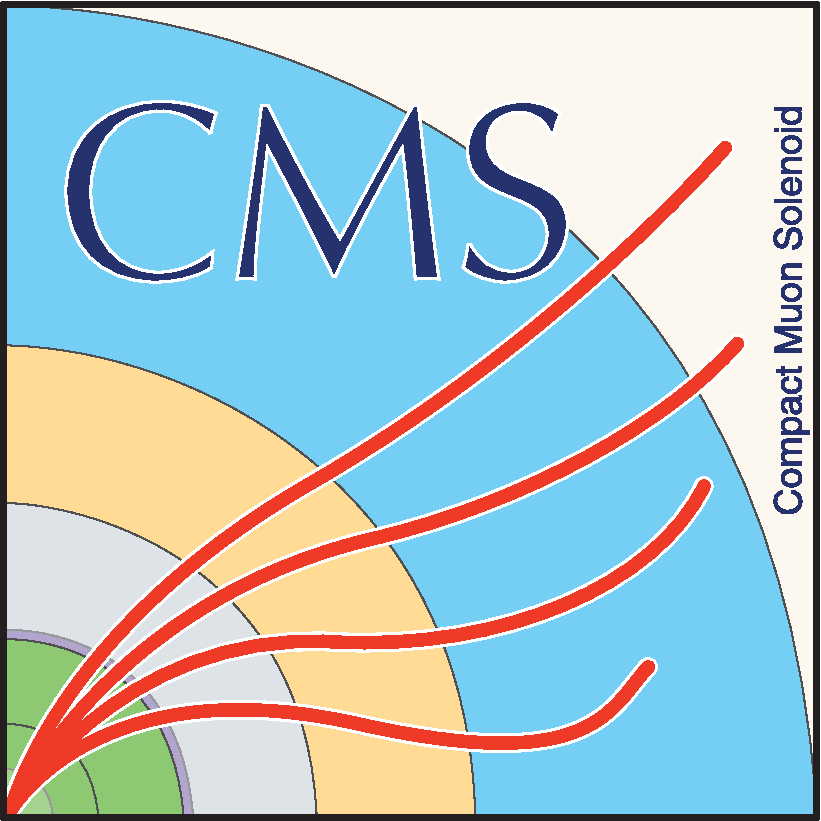
\includegraphics[height=1.25cm]{\PhDthesisdir/plots_and_images/logos/CMS_logo.pdf}
%\hfill
%
\includegraphics[trim=1cm .85cm 1cm 1cm, clip, height=1.25cm]{\PhDthesisdir/plots_and_images/logos/logo_IP2I.pdf}
%\hfill ~
%
%\vspace{-.5cm}
%\end{frame}
%
%\setcounter{framenumber}{-1}
%\begin{frame}{Lang(u)age}
%\begin{center}
%
%\textbf{\Large The slides are in English!}
%
%\begin{tikzpicture}
%\def\hsep{3}
%\def\iw{2}
%
%\def\flagw{2}
%\def\flagsep{1.5}
%
%\draw (-\hsep/2,0) node (oral_icon) {
\includegraphics[width=\iw cm]{\PhDthesisdir/plots_and_images/misc_for_slides/oral_icon.png}} ;
%\draw (+\hsep/2,0) node (slides_icon) {
\includegraphics[width=\iw cm]{\PhDthesisdir/plots_and_images/misc_for_slides/slides_icon.png}} ;
%
%\draw (oral_icon.south west) + (-120:\flagsep) node [left] (FR_flag) {
\includegraphics[width=\iw cm]{\PhDthesisdir/plots_and_images/misc_for_slides/flag-france.jpg}} ;
%\draw (slides_icon.south east) + (-60:\flagsep) node [right] (EN_flag) {
\includegraphics[width=\iw cm]{\PhDthesisdir/plots_and_images/misc_for_slides/flag-UK.png}} ;
%
%\draw [thick, -latex] (oral_icon.south west) -- (FR_flag.north east);
%\draw [thick, -latex] (slides_icon.south east) -- (EN_flag.north west);
%\end{tikzpicture}
%\end{center}
%\end{frame}

%\begin{frame}[noframenumbering] \thispagestyle{empty}
%\vspace{-.83cm}
%
%
\includegraphics[height=1.25cm]{\PhDthesisdir/plots_and_images/logos/ES-R-I_horizontal.pdf}
%\hfill
%
\includegraphics[height=1.25cm]{\PhDthesisdir/plots_and_images/logos/phast-logo.png}
%\hfill
%
\includegraphics[height=1.25cm]{\PhDthesisdir/plots_and_images/logos/Planche_UdL_LogoLyon1Sig_CoulCmjnVecto-eps-converted-to.pdf}
%\hfill
%
\includegraphics[height=1.25cm]{\PhDthesisdir/plots_and_images/logos/lycee_Raspail-Paris_14.png}
%
%\vfill
%
%%\titlepage
%\begin{center}
%{\color{CERNblue}
%
%{\large Recherche de bosons de Higgs supplémentaires de haute masse se désintégrant en paire de taus dans l'expérience CMS au LHC à l'aide du \emph{machine learning}}
%
%Soutenance de thèse de doctorat}
%
%\vfill
%
%Lucas \textsc{Torterotot}, sous la direction de Colin \textsc{Bernet}
%\end{center}
%
%\vfill
%
%~ \hfill
%
\includegraphics[height=1.25cm]{\PhDthesisdir/plots_and_images/logos/IN2P3-B_SignV_bleu-eps-converted-to.pdf}
%\hfill
%
\includegraphics[height=1.25cm]{\PhDthesisdir/plots_and_images/logos/CERN-logo.jpg}
%\hfill
%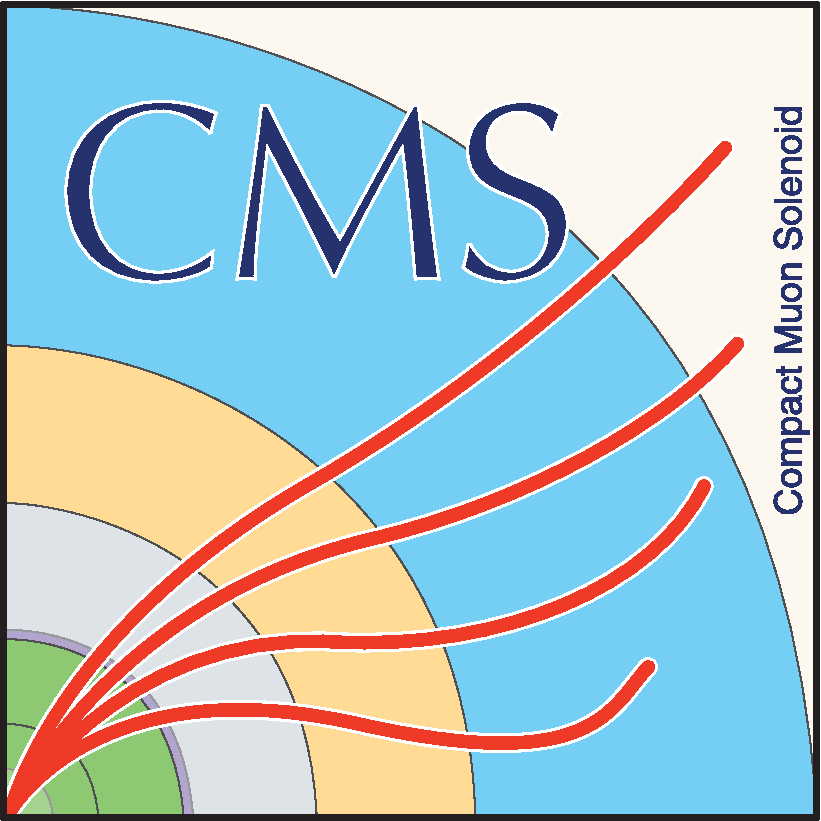
\includegraphics[height=1.25cm]{\PhDthesisdir/plots_and_images/logos/CMS_logo.pdf}
%\hfill
%
\includegraphics[trim=1cm .85cm 1cm 1cm, clip, height=1.25cm]{\PhDthesisdir/plots_and_images/logos/logo_IP2I.pdf}
%\hfill ~
%
%\vspace{-.5cm}
%\end{frame}

\begin{frame}[noframenumbering] \thispagestyle{empty}
\vspace{-.5cm}


\includegraphics[height=1.25cm]{\PhDthesisdir/plots_and_images/logos/ES-R-I_horizontal.pdf}
\hfill

\includegraphics[height=1.25cm]{\PhDthesisdir/plots_and_images/logos/phast-logo.png}
\hfill

\includegraphics[height=1.25cm]{\PhDthesisdir/plots_and_images/logos/Planche_UdL_LogoLyon1Sig_CoulCmjnVecto-eps-converted-to.pdf}
\hfill

\includegraphics[height=1.25cm]{\PhDthesisdir/plots_and_images/logos/lycee_Raspail-Paris_14.png}

\vfill

\titlepage

\vfill

~ \hfill

\includegraphics[height=1.25cm]{\PhDthesisdir/plots_and_images/logos/IN2P3-B_SignV_bleu-eps-converted-to.pdf}
\hfill

\includegraphics[height=1.25cm]{\PhDthesisdir/plots_and_images/logos/CERN-logo.jpg}
\hfill
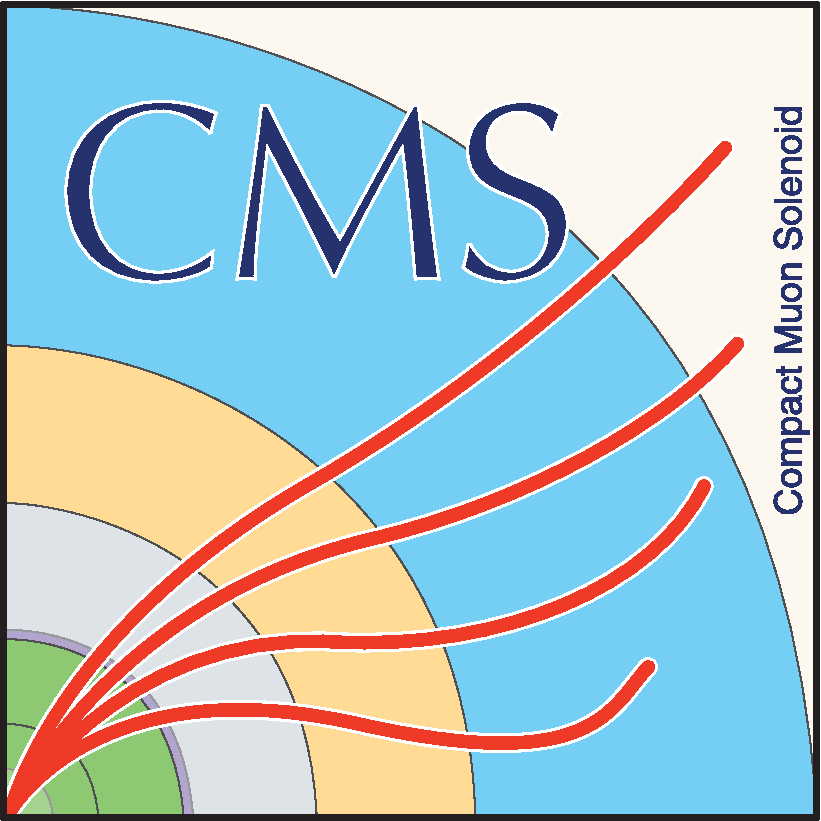
\includegraphics[height=1.25cm]{\PhDthesisdir/plots_and_images/logos/CMS_logo.pdf}
\hfill

\includegraphics[trim=1cm .85cm 1cm 1cm, clip, height=1.25cm]{\PhDthesisdir/plots_and_images/logos/logo_IP2I.pdf}
\hfill ~

%\vspace{-.5cm}
\end{frame}

\subsection*{}
\section*{Introduction}
\begin{frame}

\begin{center}
Why do we \textbf{search for...}?
\end{center}

\begin{minipage}[c]{.45\textwidth}
\begin{block}{Current standard model status}
\begin{itemize}
\item Robust and predictive (top quark, \Wboson, \Zboson\ and one Higgs boson...)
\item Still not good enough, unable to explain some observations such as:
\begin{itemize}
\item dark matter \only<2>{$\longrightarrow$}
\item matter vs antimatter asymmetry
\item naturalness problem
\item ...
\end{itemize}
\item Go beyond with a new model!
\item Consequences of this new model? \textbf{\color{ltcolorred}Test it!}
\end{itemize}
\end{block}
\end{minipage}
\hfill
\begin{minipage}[c]{.45\textwidth}
\only<2>{\begin{center}
\vspace{\baselineskip}

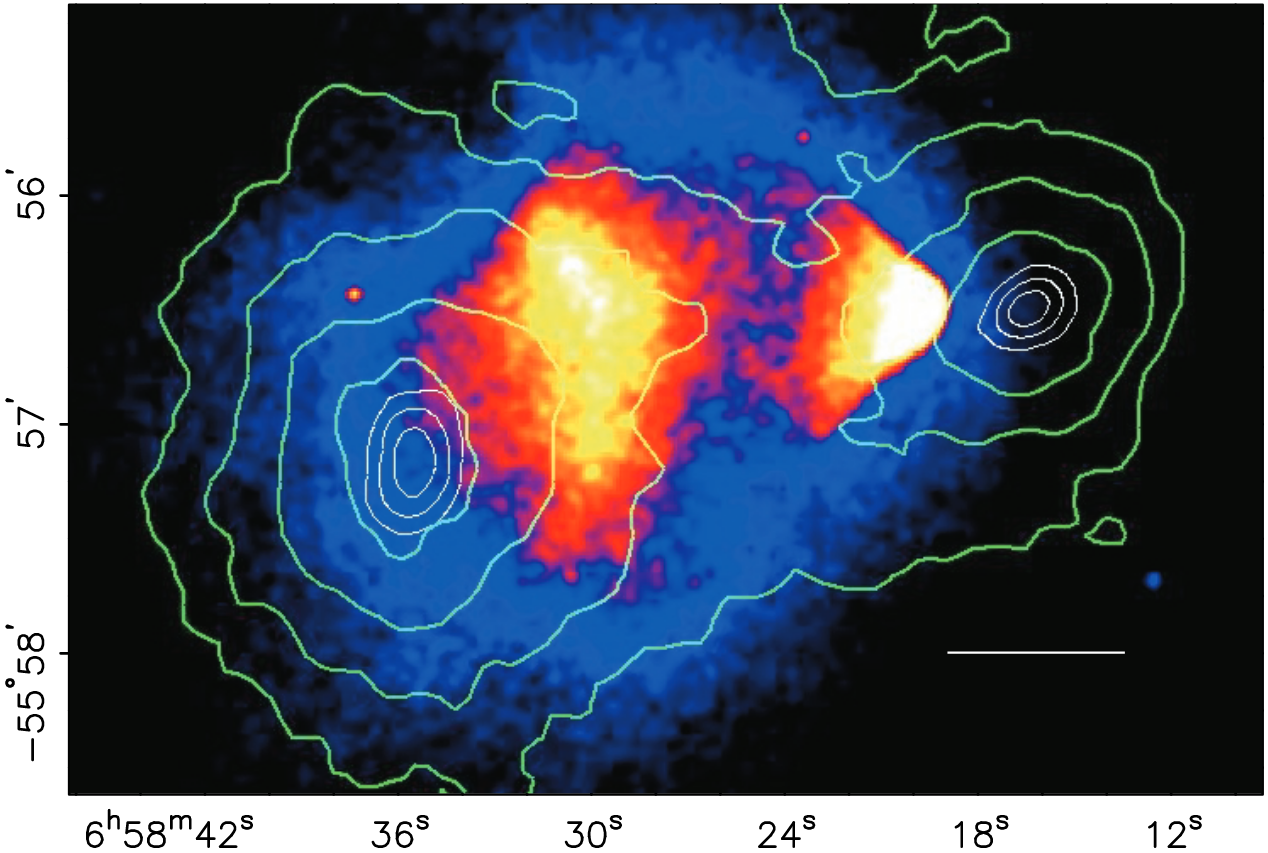
\includegraphics[width=.9\linewidth]{\PhDthesisdir/plots_and_images/from_Clowe_2006/bullet_cluster.png}

Difference due to \textbf{dark matter}!
\end{center}}
\end{minipage}
\beamercite{Clowe_2006}

\begin{tikzpicture}[overlay]
\only<2>{
\draw (.525\textwidth, .65\textheight) node (a) [above right] {Galaxies from:\vphantom{Àq}};
\draw [ltcolorred] (a.east) node [right] (b) {visible matter\vphantom{Àq}};
\draw [ltcolorgreen] (b.east) node [right] (c) {gravitational lensing\vphantom{Àq}};

\draw (.75\textwidth, .45\textheight) coordinate (b1);
\draw (.85\textwidth, .43\textheight) coordinate (b2);
\draw (.7\textwidth, .325\textheight) coordinate (c1);
\draw (.9\textwidth, .44\textheight) coordinate (c2);

\draw [ltcolorred3, thick, -latex] (b) -- (b1);
\draw [ltcolorred3, thick, -latex] (b) -- (b2);
\draw [ltcolorgreen3, thick, -latex] (c) -- (c1);
\draw [ltcolorgreen3, thick, -latex] (c) -- (c2);
}
\end{tikzpicture}
\end{frame}

\begin{frame}{Keywords in title}
\begin{center}
\small
\begin{tikzpicture}
\draw (0,0) node [below right] (t1) {Search for\vphantom{Àq}};
\draw (t1.east) node (t2) [right] {\color{ltcolorblue}\textbf{additional heavy Higgs bosons decaying to tau lepton pair}\vphantom{Àq}};
\draw (t2.east) node (t6) [right] {in the\vphantom{Àq}};
\draw (t6.east) node (t7) [right] {\color{ltcolorred}\textbf{CMS experiment at LHC}\vphantom{Àq}};

\only<2->{
\draw [thick, ltcolorblue] (t2.south east) -- (t2.south west) ;
\draw [thick, ltcolorblue, -latex] (t2.south) --+ (0,-1.5) node (l3) [below] {Part~I\vphantom{Àq}};
\draw  (l3.south) node (l3bis) {\emph{Phenomenology}};
}

\only<3->{
\draw [thick, ltcolorred] (t7.south east) -- (t7.south west) ;
\draw [thick, ltcolorred, -latex] (t7.south) --+ (0,-1.5) node (l10) [below] {Part~II\vphantom{Àq}};
\draw  (l10.south) node (l10bis) {\emph{Experimental device}};
}

\only<4->{
\draw ($(l3)!0.5!(l10)$) coordinate (middle);
\draw (middle) + (0, -1.5) node (l12) {Part~III\vphantom{Àq}};
\draw (l12.south) node (l12bis) {\emph{\HAtoTauTau\ analysis}};
\draw [thick, -latex] (l3bis) -- (l12.west) ;
\draw [thick, -latex] (l10bis) -- (l12.east) ;
}

\only<5->{
\draw (l12bis) + (0, -1.5) node {+ Part~IV: \color{ltcolorviolet}\textbf{with machine learning techniques}};
}

\draw (.5\textwidth,-.75\textheight) coordinate (a);
\end{tikzpicture}
\end{center}
\end{frame}

%\begin{frame}
%\tableofcontents 
%\end{frame}

\subsection*{}
\section{Phenomenology}
 


\subsection*{}
\section{Experimental device}
\section{The CMS detector at CERN LHC}
\subsection{CERN LHC}
%\begin{frame}
\frametitle{CERN LHC}

\begin{minipage}[c]{.45\textwidth}
\begin{center}
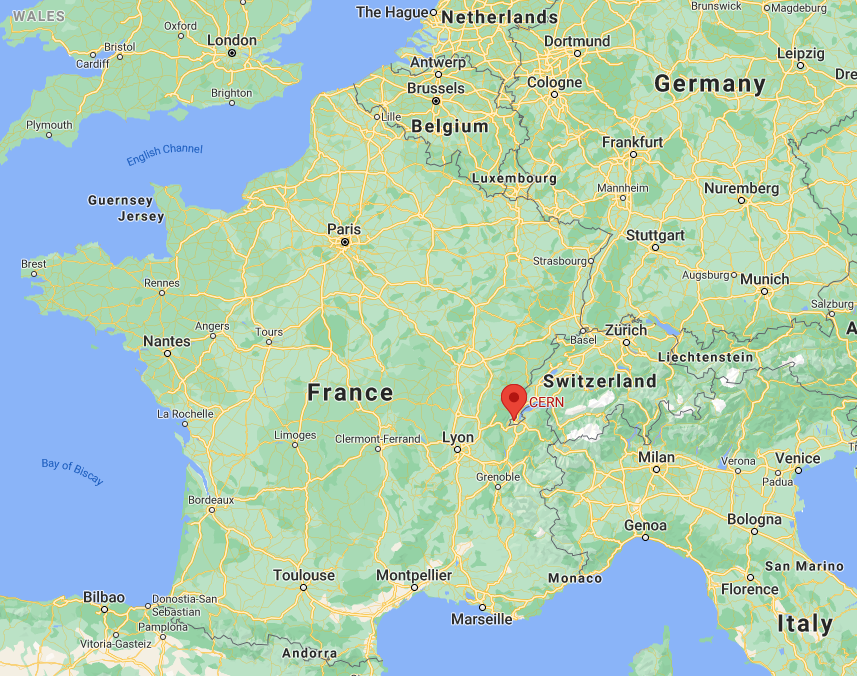
\includegraphics[width=.99\textwidth]{\PhDthesisdir/plots_and_images/CERN_and_LHC/maps-en.png}
\end{center}
\end{minipage}
\hfill
\begin{minipage}[c]{.5\textwidth}
\begin{center}
\begin{tikzpicture}
\input{\PhDthesisdir/plots_and_images/CERN_and_LHC/CERN_LHC_map-scale-bg.tex}
\fill[ltcolorred] (CMS) circle (3pt);
\draw [ltcolorred4] (CMS) node [below] {\textbf{CMS}};
\fill[ltcolorred] (ATLAS) circle (3pt);
\draw [ltcolorred4] (ATLAS) node [above] {\textbf{ATLAS}};
\fill[ltcolorred] (ALICE) circle (3pt);
\draw [ltcolorred4] (ALICE) node [above right] {\textbf{ALICE}};
\fill[ltcolorred] (LHCb) circle (3pt);
\draw [ltcolorred4] (LHCb) node [below right] {\textbf{LHCb}};
\end{tikzpicture}
\end{center}
\end{minipage}
\end{frame}


\subsection{The CMS detector}
%\begin{frame}
\frametitle{The CMS detector}
\end{frame}
\begin{frame}\addtocounter{framenumber}{-1}
\frametitle{The CMS detector -- Silicon tracker (pixels)}
\begin{center}
detects charged particles going through

\vfill

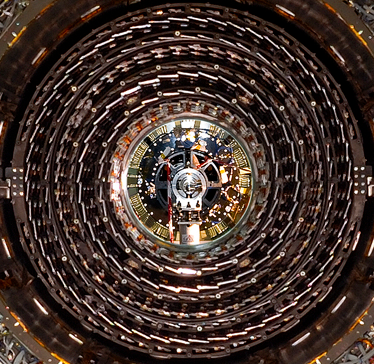
\includegraphics[width=\textwidth,height=0.75\textheight,keepaspectratio]{\PhDthesisdir/slides/LHC-CMS/CMS/CMS_zoomout_pictures/CMS_slice_photo_1-trk1.png}

\vfill

$\longleftarrow \SI{1}{\meter} \longrightarrow$
\end{center}
\end{frame}
\begin{frame}\addtocounter{framenumber}{-1}
\frametitle{The CMS detector -- Silicon tracker (strips)}
\begin{center}
detects charged particles going through

\vfill

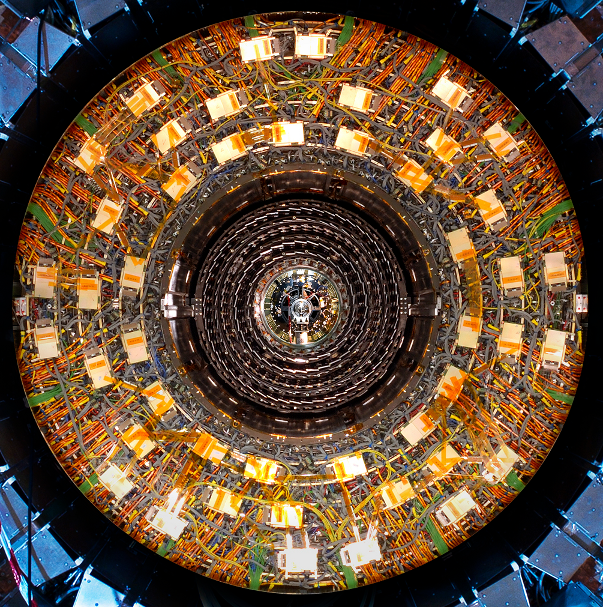
\includegraphics[width=\textwidth,height=0.75\textheight,keepaspectratio]{\PhDthesisdir/slides/LHC-CMS/CMS/CMS_zoomout_pictures/CMS_slice_photo_2-trk2.png}

\vfill

$\longleftarrow \SI{2}{\meter} \longrightarrow$
\end{center}
\end{frame}
\begin{frame}\addtocounter{framenumber}{-1}
\frametitle{The CMS detector -- Electromagnetic calorimeter (ECAL)}
\begin{center}
stops photons and electrons, measure their energies

\vfill

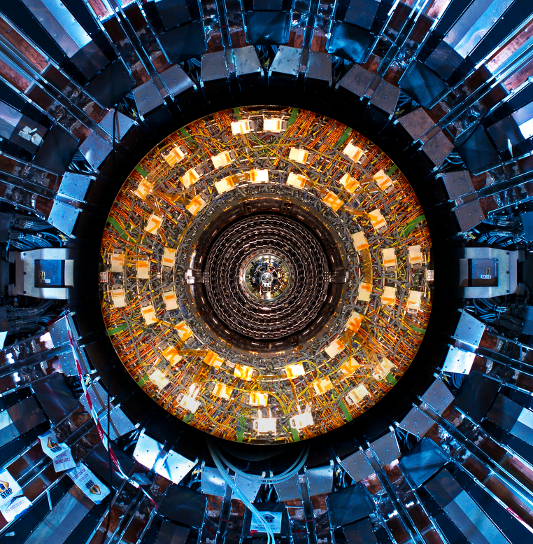
\includegraphics[width=\textwidth,height=0.75\textheight,keepaspectratio]{\PhDthesisdir/slides/LHC-CMS/CMS/CMS_zoomout_pictures/CMS_slice_photo_3-ECAL.png}

\vfill

$\longleftarrow \SI{3}{\meter} \longrightarrow$
\end{center}
\end{frame}
\begin{frame}\addtocounter{framenumber}{-1}
\frametitle{The CMS detector -- Hadron calorimeter (HCAL)}
\begin{center}
stops hadrons (protons, neutrons, ...), measure their energies

\vfill

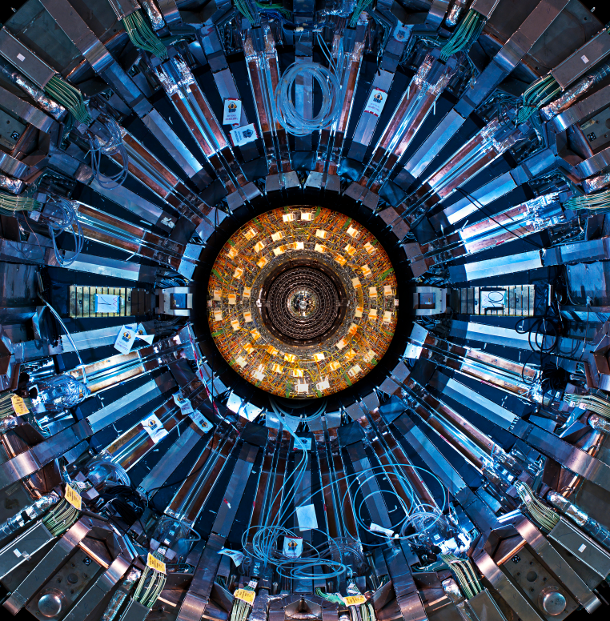
\includegraphics[width=\textwidth,height=0.75\textheight,keepaspectratio]{\PhDthesisdir/slides/LHC-CMS/CMS/CMS_zoomout_pictures/CMS_slice_photo_4-HCAL.png}

\vfill

$\longleftarrow \SI{5}{\meter} \longrightarrow$
\end{center}
\end{frame}
\begin{frame}\addtocounter{framenumber}{-1}
\frametitle{The CMS detector -- Superconducting solenoid}
\begin{center}
creates a \SI{4}{\tesla} magnetic field which bends charged particles trajectories

\vfill

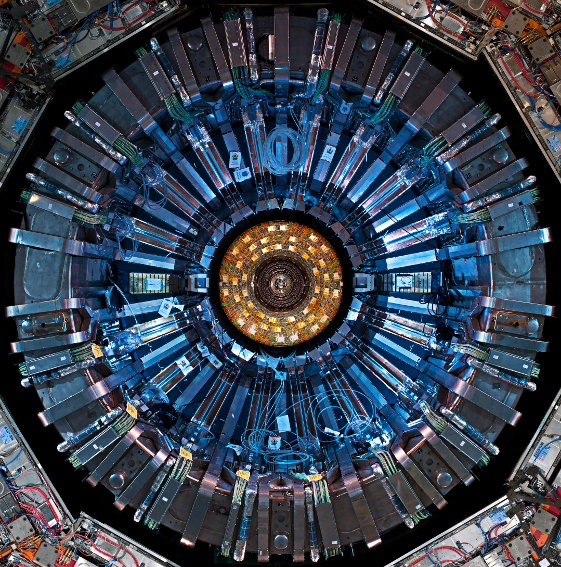
\includegraphics[width=\textwidth,height=0.75\textheight,keepaspectratio]{\PhDthesisdir/slides/LHC-CMS/CMS/CMS_zoomout_pictures/CMS_slice_photo_5-solenoid.png}

\vfill

$\longleftarrow \SI{7}{\meter} \longrightarrow$
\end{center}
\end{frame}
\begin{frame}\addtocounter{framenumber}{-1}
\frametitle{The CMS detector -- Muon system}
\begin{center}
detects muons going through

\vfill

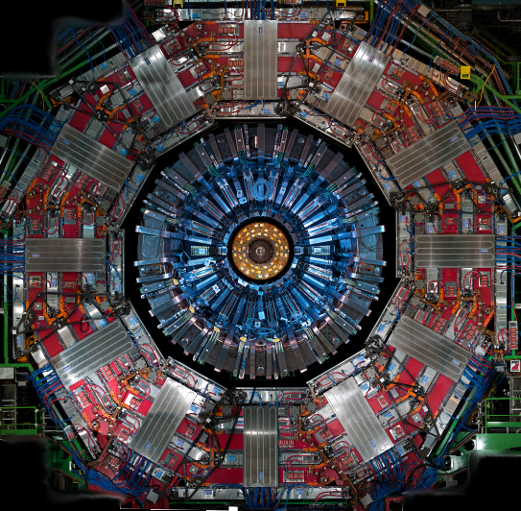
\includegraphics[width=\textwidth,height=0.75\textheight,keepaspectratio]{\PhDthesisdir/slides/LHC-CMS/CMS/CMS_zoomout_pictures/CMS_slice_photo_6-muons.png}

\vfill

$\longleftarrow \SI{15}{\meter} \longrightarrow$
\end{center}
\end{frame}
%\begin{frame}\addtocounter{framenumber}{-1}
\frametitle{The CMS detector}
\begin{center}
\vphantom{detects muons going through}

\vfill

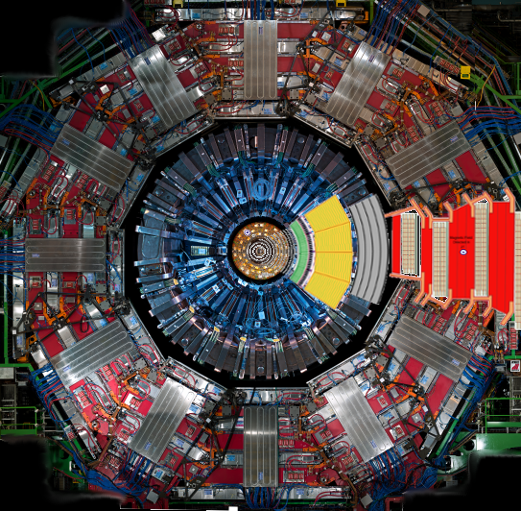
\includegraphics[width=\textwidth,height=0.75\textheight,keepaspectratio]{\PhDthesisdir/plots_and_images/CMS_slices/own/slice_on_photo.tex}

\vfill

$\longleftarrow \SI{15}{\meter} \longrightarrow$
\end{center}
\end{frame}
\begin{frame}
\begin{minipage}[t]{.6\textwidth}
\begin{figure}
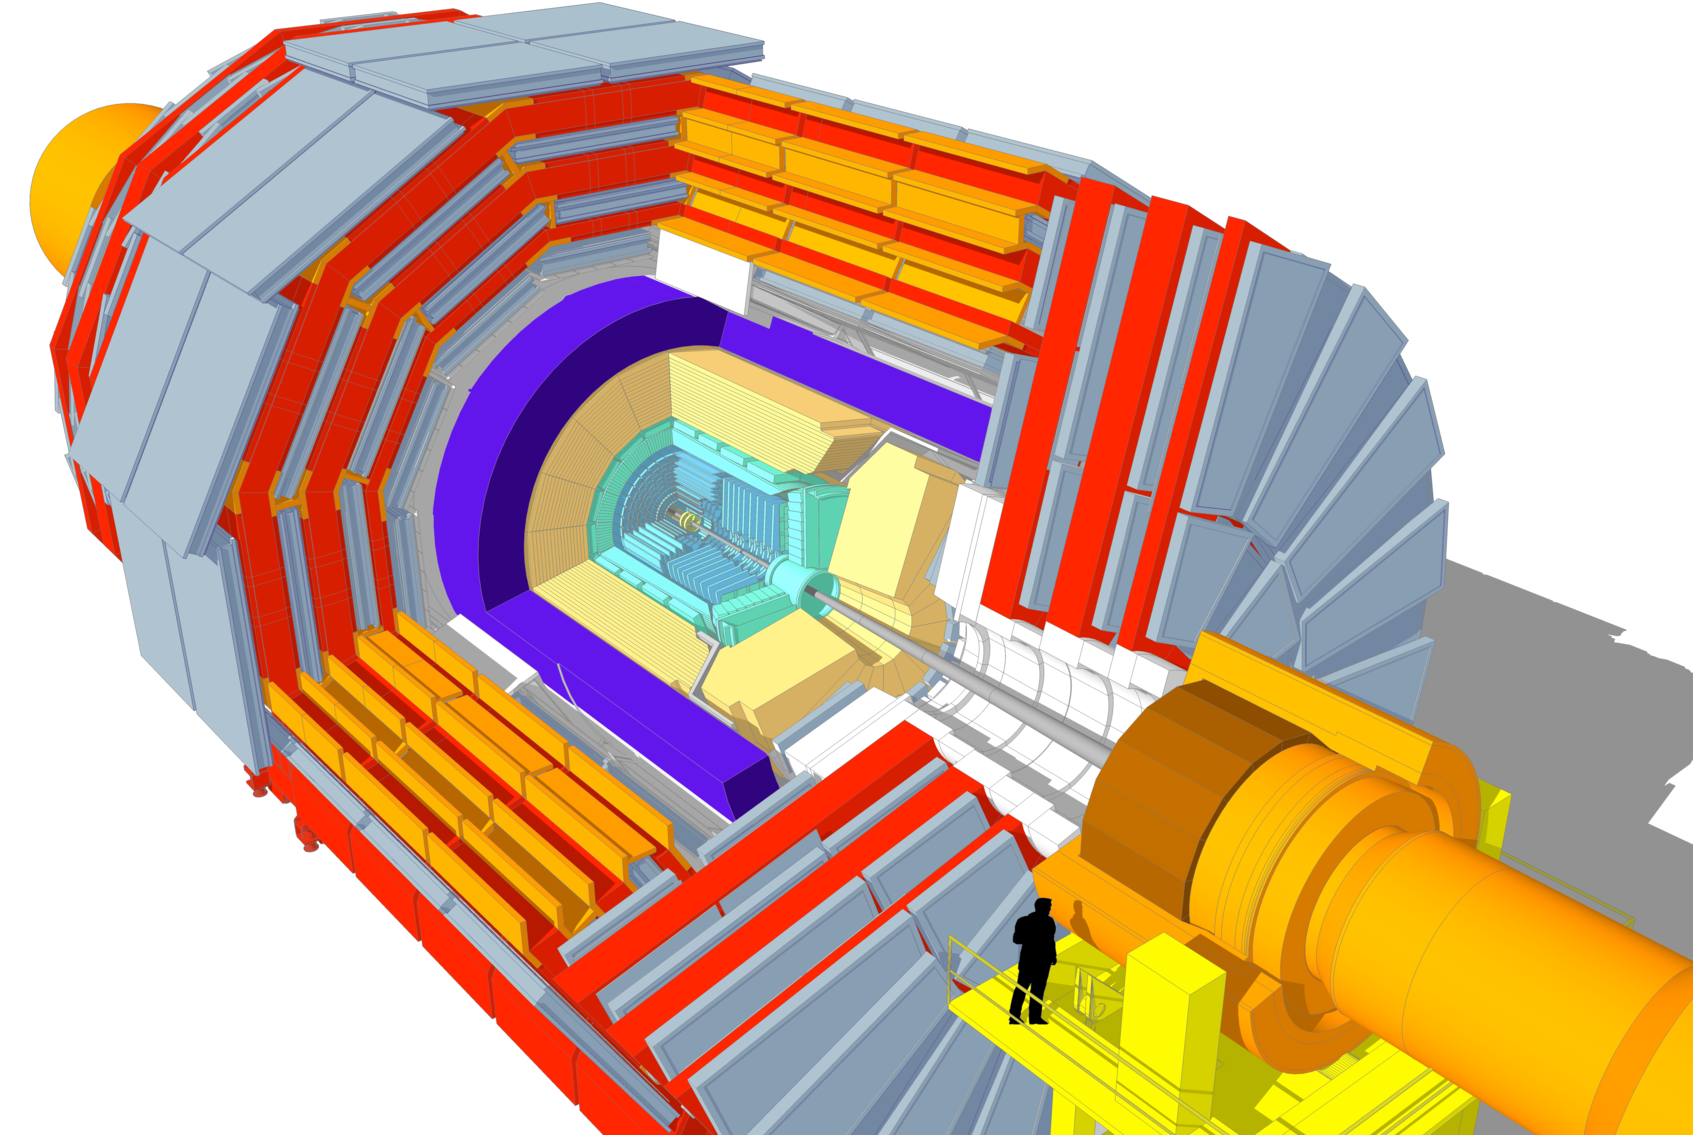
\includegraphics[width=\textwidth,height=\graphh,keepaspectratio]{\PhDthesisdir/plots_and_images/CMS_slices/from_CMS_document_11982-v2/small_cms_full.png}
\end{figure}
\end{minipage}
\hfill\begin{minipage}[t]{.35\textwidth}
\begin{block}{CMS detector}
\begin{itemize}
\item Mass: $\sim\SI{14000}{t}$, $\num{12500}$ only for red part
\item Diameter: \SI{15}{\meter}
\item Length: \SI{28.7}{\meter}
\end{itemize}
\end{block}

\begin{block}{}
$\Rightarrow$ How to \emph{see} the particles?
\end{block}
\end{minipage}
\end{frame}

\begin{frame}
\addtocounter{framenumber}{-1}
%\transdissolve
\begin{minipage}[t]{.6\textwidth}
\begin{figure}
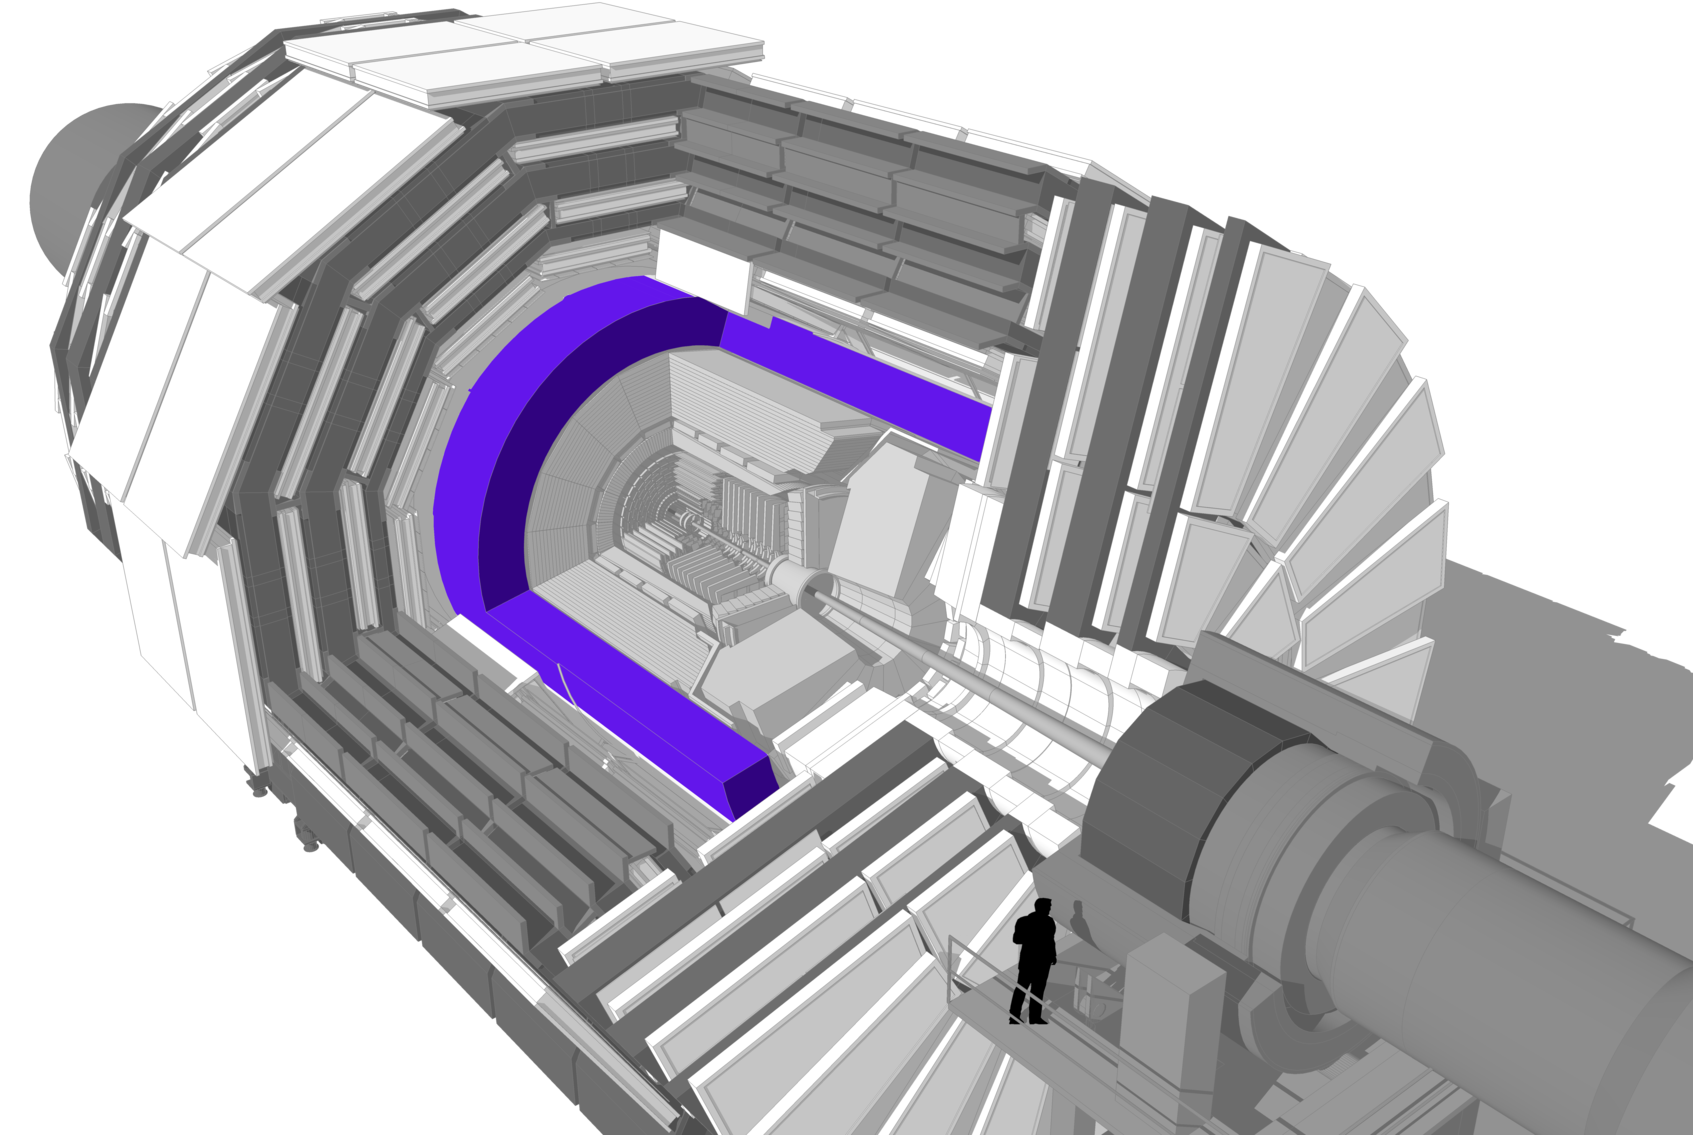
\includegraphics[width=\textwidth,height=\graphh,keepaspectratio]{\PhDthesisdir/plots_and_images/CMS_slices/from_CMS_document_11982-v2/small_cms_solenoid.png}
\end{figure}
\end{minipage}
\hfill\begin{minipage}[t]{.35\textwidth}
\begin{block}{Solenoid}
\begin{itemize}
\item Niobium titanium coil
\item Superconducting
\item $\sim\SI{18000}{\ampere}$
\item \SI{4}{\tesla} in the inner volume
\end{itemize}
\end{block}

\begin{block}{}
$\Rightarrow$ Bends charged particles trajectories in the transverse plane
\end{block}
\end{minipage}
\end{frame}

\begin{frame}
\addtocounter{framenumber}{-1}
%\transdissolve
\begin{minipage}[t]{.6\textwidth}
\begin{figure}
\includegraphics[width=\textwidth,height=\graphh,keepaspectratio]{\PhDthesisdir/plots_and_images/CMS_slices/from_CMS_document_11982-v2/small_cms_tracker.png}
\end{figure}
\end{minipage}
\hfill\begin{minipage}[t]{.35\textwidth}
\begin{block}{Tracker}
\begin{itemize}
\item Inner: pixels ($\num{100}\times\SI{150}{\micro\meter^2}$, $\sim\SI{1.9}{\meter^2}$, $\sim\SI{124}{M}$ channels
\item Outer: microstrips ($\num{80}-\SI{180}{\micro\meter}$) $\sim\SI{200}{\meter^2}$ $\sim\SI{9.6}{M}$ channels
\end{itemize}
\end{block}

\begin{block}{}
$\Rightarrow$ Charged particles leave hits when going through
\end{block}
\end{minipage}
\end{frame}

\begin{frame}
\addtocounter{framenumber}{-1}
%\transdissolve
\begin{minipage}[t]{.6\textwidth}
\begin{figure}
\includegraphics[width=\textwidth,height=\graphh,keepaspectratio]{\PhDthesisdir/plots_and_images/CMS_slices/from_CMS_document_11982-v2/small_cms_ecal.png}
\end{figure}
\end{minipage}
\hfill\begin{minipage}[t]{.35\textwidth}
\begin{block}{Electromagnetic CALorimeter}
\begin{itemize}
\item $\sim\num{76000}$ scintillating \ce{PbWO4} crystals
\end{itemize}
\end{block}

\begin{block}{}
$\Rightarrow$ electrons and photons are stopped, energy deposits
\end{block}
\end{minipage}
\end{frame}

\begin{frame}
\addtocounter{framenumber}{-1}
%\transdissolve
\begin{minipage}[t]{.6\textwidth}
\begin{figure}
\includegraphics[width=\textwidth,height=\graphh,keepaspectratio]{\PhDthesisdir/plots_and_images/CMS_slices/from_CMS_document_11982-v2/small_cms_hcal.png}
\end{figure}
\end{minipage}
\hfill\begin{minipage}[t]{.35\textwidth}
\begin{block}{Hadronic CALorimeter (yellow)}
\begin{itemize}
\item brass + plastic scintillator, $\sim\num{7000}$ channels
\end{itemize}
\end{block}

\begin{block}{Forward CALorimeter (orange)}
\begin{itemize}
\item steel + quartz fibres, $\sim\num{2000}$ channels
\end{itemize}
\end{block}

\begin{block}{}
$\Rightarrow$ hadrons are stopped, energy deposits
\end{block}
\end{minipage}
\end{frame}

\begin{frame}
\addtocounter{framenumber}{-1}
%\transdissolve
\begin{minipage}[t]{.6\textwidth}
\begin{figure}
\includegraphics[width=\textwidth,height=\graphh,keepaspectratio]{\PhDthesisdir/plots_and_images/CMS_slices/from_CMS_document_11982-v2/small_cms_muons.png}
\end{figure}
\end{minipage}
\hfill\begin{minipage}[t]{.35\textwidth}
\begin{block}{Steel return yoke (red)}
\begin{itemize}
\item allows for \SI{2}{\tesla} magnetic field around the solenoid
\end{itemize}
\end{block}

\begin{block}{Muon chambers (blue-gray)}
\begin{itemize}
\item Barrel: \num{250} drift tubes, \num{480} resistive plate chambers
\item Endcaps: \num{540} cathode strip, \num{576} resistive plate chambers
\end{itemize}
\end{block}

\begin{block}{}
$\Rightarrow$ charged particles leave hits when going through (only muons do)
\end{block}
\vspace{-2\baselineskip}
\end{minipage}
\end{frame}

\begin{frame}
\addtocounter{framenumber}{-1}
%\transdissolve
\begin{minipage}[t]{.6\textwidth}
\begin{figure}
\includegraphics[width=\textwidth,height=\graphh,keepaspectratio]{\PhDthesisdir/plots_and_images/CMS_slices/from_CMS_document_11982-v2/small_cms_full_no_violet_solen.png}
\end{figure}
\end{minipage}
\hfill\begin{minipage}[t]{.35\textwidth}
\begin{block}{Sensitive parts of CMS}
Combine sub-detectors signals to determine which particles were there!
\end{block}
\end{minipage}
\end{frame}
\begin{frame}
\transdissolve
\transduration{0}
\end{frame}

\begin{frame}
\transwipe
\transduration{0}
\begin{center}
\includegraphics[width=\textwidth,height=\graphh,keepaspectratio]{\PhDthesisdir/plots_and_images/CMS_slices/own/cms_slice_CMS_parts/1-only_cms_size.tex}
\end{center}
\end{frame}

\begin{frame}
\addtocounter{framenumber}{-1}
\transdissolve[duration=2]
\transduration{0}
\begin{center}
\includegraphics[width=\textwidth,height=\graphh,keepaspectratio]{\PhDthesisdir/plots_and_images/CMS_slices/own/cms_slice_CMS_parts/2-add_trk.tex}
\end{center}
\end{frame}

\begin{frame}
\addtocounter{framenumber}{-1}
\transdissolve[duration=2]
\transduration{0}
\begin{center}
\includegraphics[width=\textwidth,height=\graphh,keepaspectratio]{\PhDthesisdir/plots_and_images/CMS_slices/own/cms_slice_CMS_parts/3-add_ECAL.tex}
\end{center}
\end{frame}

\begin{frame}
\addtocounter{framenumber}{-1}
\transdissolve[duration=2]
\transduration{0}
\begin{center}
\includegraphics[width=\textwidth,height=\graphh,keepaspectratio]{\PhDthesisdir/plots_and_images/CMS_slices/own/cms_slice_CMS_parts/4-add_HCAL.tex}
\end{center}
\end{frame}

\begin{frame}
\addtocounter{framenumber}{-1}
\transdissolve[duration=2]
\transduration{0}
\begin{center}
\includegraphics[width=\textwidth,height=\graphh,keepaspectratio]{\PhDthesisdir/plots_and_images/CMS_slices/own/cms_slice_CMS_parts/5-add_solen.tex}
\end{center}
\end{frame}

%\begin{frame}
%\addtocounter{framenumber}{-1}
%\transdissolve
%\transduration{0}
%\begin{center}
%\includegraphics[width=\textwidth,height=\graphh,keepaspectratio]{\PhDthesisdir/plots_and_images/CMS_slices/own/cms_slice_CMS_parts/6-1-add_iron_RY.tex}
%\end{center}
%\end{frame}
%
%\begin{frame}
%\addtocounter{framenumber}{-1}
%\transdissolve
%\transduration{0}
%\begin{center}
%\includegraphics[width=\textwidth,height=\graphh,keepaspectratio]{\PhDthesisdir/plots_and_images/CMS_slices/own/cms_slice_CMS_parts/6-2-add_muon1.tex}
%\end{center}
%\end{frame}
%
%\begin{frame}
%\addtocounter{framenumber}{-1}
%\transdissolve
%\transduration{0}
%\begin{center}
%\includegraphics[width=\textwidth,height=\graphh,keepaspectratio]{\PhDthesisdir/plots_and_images/CMS_slices/own/cms_slice_CMS_parts/6-3-add_muon2.tex}
%\end{center}
%\end{frame}
%
%\begin{frame}
%\addtocounter{framenumber}{-1}
%\transdissolve
%\transduration{0}
%\begin{center}
%\includegraphics[width=\textwidth,height=\graphh,keepaspectratio]{\PhDthesisdir/plots_and_images/CMS_slices/own/cms_slice_CMS_parts/6-4-add_muon3.tex}
%\end{center}
%\end{frame}

\begin{frame}
\addtocounter{framenumber}{-1}
\transdissolve[duration=2]
\transduration{0}
\begin{center}
\includegraphics[width=\textwidth,height=\graphh,keepaspectratio]{\PhDthesisdir/plots_and_images/CMS_slices/own/cms_slice_CMS_parts/6-5-add_muon4.tex}
\end{center}
\end{frame}

%\begin{frame}
%\addtocounter{framenumber}{-1}
%\transdissolve[duration=2]
%\transduration{0}
%\begin{center}
%\includegraphics[width=\textwidth,height=\graphh,keepaspectratio]{\PhDthesisdir/plots_and_images/CMS_slices/own/cms_slice_CMS_parts/7-add_B_field.tex}
%\end{center}
%\end{frame}

\begin{frame}
\addtocounter{framenumber}{-1}
\transdissolve[duration=2]
\transduration{0}
\begin{center}
\includegraphics[width=\textwidth,height=\graphh,keepaspectratio]{\PhDthesisdir/plots_and_images/CMS_slices/own/cms_slice_particles_appear/0-nothing.tex}
\end{center}
\end{frame}

%\begin{frame}
%\addtocounter{framenumber}{-1}
%\transwipe
%\transduration{0}
%\begin{center}
%\includegraphics[width=\textwidth,height=\graphh,keepaspectratio]{\PhDthesisdir/plots_and_images/CMS_slices/own/cms_slice_particles_appear/1-up_to_CH.tex}
%\end{center}
%\end{frame}
%
%\begin{frame}
%\addtocounter{framenumber}{-1}
%\transwipe
%\transduration{0}
%\begin{center}
%\includegraphics[width=\textwidth,height=\graphh,keepaspectratio]{\PhDthesisdir/plots_and_images/CMS_slices/own/cms_slice_particles_appear/2-up_to_NH.tex}
%\end{center}
%\end{frame}
%
%\begin{frame}
%\addtocounter{framenumber}{-1}
%\transwipe
%\transduration{0}
%\begin{center}
%\includegraphics[width=\textwidth,height=\graphh,keepaspectratio]{\PhDthesisdir/plots_and_images/CMS_slices/own/cms_slice_particles_appear/3-up_to_photon.tex}
%\end{center}
%\end{frame}
%
%\begin{frame}
%\addtocounter{framenumber}{-1}
%\transwipe
%\transduration{0}
%\begin{center}
%\includegraphics[width=\textwidth,height=\graphh,keepaspectratio]{\PhDthesisdir/plots_and_images/CMS_slices/own/cms_slice_particles_appear/4-up_to_ele.tex}
%\end{center}
%\end{frame}

\begin{frame}
\addtocounter{framenumber}{-1}
\transwipe
\begin{center}
\includegraphics[width=\textwidth,height=\graphh,keepaspectratio]{\PhDthesisdir/plots_and_images/CMS_slices/own/all_ptcs.tex}
\end{center}
\end{frame}
%\begin{frame}
\frametitle{Neutrinos and missing transverse energy (MET)}

\begin{center}
\begin{tikzpicture}
\input{\PhDthesisdir/tex/Event_displays/macro_defs.tex}

\clip (-\graphw/2,-\graphh/2) rectangle (\graphw/2,\graphh/2);

\printjetnolabel{60}
\printjetnolabel{40}

%\draw [thick, -latex, ltcolorred] (0,0)--+(-130:\HCALrout) node [below] {\vMET};

\fill (0,0) circle (2pt);
\end{tikzpicture}
\end{center}

\end{frame}

\begin{frame}\addtocounter{framenumber}{-1}
\frametitle{Neutrinos and missing transverse energy (MET)}

\begin{center}
\begin{tikzpicture}
\input{\PhDthesisdir/tex/Event_displays/macro_defs.tex}

\clip (-\graphw/2,-\graphh/2) rectangle (\graphw/2,\graphh/2);

\printjetnolabel{60}
\printjetnolabel{40}

\draw [thick, -latex, ltcolorred] (0,0)--+(-130:\HCALrout) node [below] {\vMET};

\fill (0,0) circle (2pt);
\end{tikzpicture}
\end{center}

\end{frame}

%\begin{frame}
\frametitle{Event display: $\higgs\to\tau\tau\to\mu\tauh$ candidate}
\vfill
\includegraphics[width=\graphw,height=\graphh,keepaspectratio]{\PhDthesisdir/tex/slides/SM_MSSM_HTT_pheno/event_display/Event_1429090375_xy_white_struct_tracks.png}

\vfill

{\tiny
CMS record, Aug. 18, 2012, 14:37:39.352716 GMT
\qquad
Run 201191, Event 1429090375, LS 1071, xy plane.
}
\end{frame}


%\subsection*{Jet energy calibration}

\begin{frame}
\begin{minipage}[t]{.45\textwidth}
\begin{center}
\manip Niveaux de connaissance

\vspace{.5\baselineskip}

\begin{tabular}{rl}
particule & (\ptcl)\\
reconstruit & (\reco)\\
corrigé & (\cali)
\end{tabular}
\end{center}
\end{minipage}
\hfill\pause
\begin{minipage}[t]{.45\textwidth}
\begin{center}
\manip Réponse d'un jet
\begin{equation*}
R = \frac{\pT}{\pT_\ptcl}
\end{equation*}
\end{center}
\end{minipage}
\end{frame}


\begin{frame}[t]
%\transdissolve
\large
\includegraphics[width=\textwidth]{\PhDthesisdir/plots_and_images/from_JERC_RunI/CMS-JME-13-004_Figure_002-FR-TeX-sequential_for_slides/1.tex}

\vfill

\includegraphics[height = \textheight/2]{\PhDthesisdir/plots_and_images/from_JERC_RunI/response_evolution_1.png}
\hfill
\includegraphics[height = \textheight/2]{\PhDthesisdir/plots_and_images/from_JERC_RunI/response_evolution_3.png}
\end{frame}

\begin{frame}[t]
\addtocounter{framenumber}{-1}
%\transdissolve
\large
\includegraphics[width=\textwidth]{\PhDthesisdir/plots_and_images/from_JERC_RunI/CMS-JME-13-004_Figure_002-FR-TeX-sequential_for_slides/2.tex}

\vfill

\includegraphics[height = \textheight/2]{\PhDthesisdir/plots_and_images/from_JERC_RunI/response_evolution_1.png}
\hfill
\includegraphics[height = \textheight/2]{\PhDthesisdir/plots_and_images/from_JERC_RunI/response_evolution_3.png}
\end{frame}

\begin{frame}[t]
\addtocounter{framenumber}{-1}
%\transdissolve
\large
\includegraphics[width=\textwidth]{\PhDthesisdir/plots_and_images/from_JERC_RunI/CMS-JME-13-004_Figure_002-FR-TeX-sequential_for_slides/3.tex}

\vfill

\includegraphics[height = \textheight/2]{\PhDthesisdir/plots_and_images/from_JERC_RunI/response_evolution_1.png}
\hfill
\includegraphics[height = \textheight/2]{\PhDthesisdir/plots_and_images/from_JERC_RunI/response_evolution_2.png}
\hfill
\includegraphics[height = \textheight/2]{\PhDthesisdir/plots_and_images/from_JERC_RunI/response_evolution_3.png}
\end{frame}

\begin{frame}[t]
\addtocounter{framenumber}{-1}
%\transdissolve
\large
\includegraphics[width=\textwidth]{\PhDthesisdir/plots_and_images/from_JERC_RunI/CMS-JME-13-004_Figure_002-FR-TeX-sequential_for_slides/4.tex}

\vfill

\includegraphics[height = \textheight/2]{\PhDthesisdir/plots_and_images/from_CMS-DP-2020-019/simulated_jet_response_2016.png}
\hfill
\includegraphics[height = \textheight/2]{\PhDthesisdir/plots_and_images/from_CMS-DP-2020-019/simulated_jet_response_2017.png}
\hfill
\includegraphics[height = \textheight/2]{\PhDthesisdir/plots_and_images/from_CMS-DP-2020-019/simulated_jet_response_2018.png}
\end{frame}

\begin{frame}[t]
\addtocounter{framenumber}{-1}
%\transdissolve
\large
\includegraphics[width=\textwidth]{\PhDthesisdir/plots_and_images/from_JERC_RunI/CMS-JME-13-004_Figure_002-FR-TeX-sequential_for_slides/5.tex}
\end{frame}

\begin{frame}[t]
\addtocounter{framenumber}{-1}
%\transdissolve
\large
\includegraphics[width=\textwidth]{\PhDthesisdir/plots_and_images/from_JERC_RunI/CMS-JME-13-004_Figure_002-FR-TeX-sequential_for_slides/6.tex}

\vfill

\includegraphics[height = \textheight/2]{\PhDthesisdir/plots_and_images/from_CMS-DP-2020-019/absolute_pT_residual_2016.png}
\hfill
\includegraphics[height = \textheight/2]{\PhDthesisdir/plots_and_images/from_CMS-DP-2020-019/absolute_pT_residual_2017.png}
\hfill
\includegraphics[height = \textheight/2]{\PhDthesisdir/plots_and_images/from_CMS-DP-2020-019/absolute_pT_residual_2018.png}
\end{frame}

\begin{frame}[t]
\addtocounter{framenumber}{-1}
%\transdissolve
\large
\includegraphics[width=\textwidth]{\PhDthesisdir/plots_and_images/from_JERC_RunI/CMS-JME-13-004_Figure_002-FR-TeX.tex}

\vfill

\begin{center}
\includegraphics[height = \textheight/2]{\PhDthesisdir/plots_and_images/from_JERC_RunI/Figure_030-a.png}
\end{center}
\end{frame}



\input{\PhDthesisdir/tex/slides/JERC/JEC_Principe/Gamma_plus_jets_events.tex}
\input{\PhDthesisdir/tex/slides/JERC/JEC_Principe/Rbal_alpha_and_RMPF.tex}
\input{\PhDthesisdir/tex/slides/JERC/JEC_results/JEC_plots.tex}

\input{\PhDthesisdir/slides/JERC/JER_Principe/JER_formulas.tex}
\input{\PhDthesisdir/slides/JERC/JER_results/JER_plots.tex}


\subsection*{}
\section{\HAtoTauTau\ analysis}
 


\subsection*{}
\section*{}
\begin{frame}

\begin{minipage}[t]{.45\textwidth}
\manip Remember: invariant mass not fully available:
\submanip neutrinos in di-\tau\ events.
\pause
\begin{block}{What's here}
\begin{center}
{\small (e.g. VBF Higgs production + decay to \tau\tau, \mu\tauh\ channel)}

\vspace{.5\baselineskip}

    \begin{tikzpicture}[scale=.8]
        \clip (-.5\linewidth,-.3\linewidth) rectangle (.5\linewidth,.3\linewidth);

        %\drawCMS

        %\printantimuondeposit{21}{50}
        \printantimuonnolabel{21}{50}
        \draw (55:\ECALrin) node {\color{\muoncolor}\mu};
        
        \printneutrinonolabel{52}
        \draw (60:\HCALrin) node {\antinutau};
        \printneutrinonolabel{45}
        \draw (35:\HCALrin) node {\numu};


        %\printjetdeposit{50}{170}
        \printjetnolabel{50}{170}
        \draw (170:\HCALrout) node {\color{\jetcolor}jet};

        %\printbigjetdeposit{150}{-50}
        \printbigjetnolabel{150}{-50}
        \draw (-40:\HCALrout) node {\color{\jetcolor}jet};

        %\printtauhdeposit{15}{-150}
        \printtauhnolabel{15}{-150}
        \draw (-135:\HCALrin) node {\color{\tauhcolor}\tauh};
        
        \printneutrinonolabel{-150}
        \draw (-155:\HCALrout) node {\nutau};
    \end{tikzpicture}
\end{center}
\end{block}

\only<4->{
\manip It would be great to have a di-\tau\ mass estimator!
\submanip What about \emph{\textbf{machine learning}}?
}
\end{minipage}
\hfill
\begin{minipage}[t]{.45\textwidth}
\vspace{-\baselineskip}
\begin{block}{What CMS sees: no neutrinos but \MET}
\begin{center}
\begin{center}
    \begin{tikzpicture}[scale=.45]
        \clip (0,0) circle (\muonroutd);

        \drawCMS

        \printantimuondeposit{21}{50}
        \printantimuontrk{21}{50}
%        \printantimuon{21}{50}

        \printjetdeposit{50}{170}
        \printjettrk{50}{170}
%        \printjetnolabel{50}{170}

        \printbigjetdeposit{150}{-50}
        \printbigjettrk{150}{-50}
%        \printbigjetnolabel{150}{-50}

        \printtauhdeposit{15}{-150}
        \printtauhtrk{15}{-150}
%        \printtauh{15}{-150}
        
        \draw [thick, ltcolorred, -latex] (0,0) --+ (75:.3\linewidth) node [right] {\vMET};
    \end{tikzpicture}
\end{center}
\end{center}
\end{block}
\end{minipage}

\begin{tikzpicture}[overlay, remember picture]
\only<-2>{
\fill [white] (.5\textwidth, -.1\textheight) rectangle (1.1\textwidth, .975\textheight);
}
\end{tikzpicture}
\end{frame}

\subsection*{}
\section{Machine learning}
\subsection{Event topology}
\begin{frame}%{Event topology (no PU considered)}

\begin{minipage}[c]{.275\textwidth}
\begin{block}{Higgs production}
\begin{center}
\small

\vspace{\baselineskip}

\input{\PhDthesisdir/plots_and_images/Feynman_diagrams/H_production/smalls_for_beamer/fgraph-gg_loop_H.tex}

\vspace{2\baselineskip}

\input{\PhDthesisdir/plots_and_images/Feynman_diagrams/H_production/smalls_for_beamer/fgraph-bg_b_bH.tex}

\vspace{2\baselineskip}

\input{\PhDthesisdir/plots_and_images/Feynman_diagrams/H_production/smalls_for_beamer/fgraph-gg_Hbb.tex}

\vspace{\baselineskip}

...
\end{center}
\end{block}
\end{minipage}
\hfill%\pause
\begin{minipage}[c]{.04\textwidth}
\begin{center}
\large$\times$
\end{center}
\end{minipage}
\hfill
\begin{minipage}[c]{.275\textwidth}
\begin{block}{$\Higgs\to\tau\tau$}
\begin{center}
\vspace{\baselineskip}
\input{\PhDthesisdir/plots_and_images/Feynman_diagrams/fgraph-H-tautau_small_beamer.tex}
\vspace{\baselineskip}
\end{center}
\end{block}
\end{minipage}
\hfill%\pause
\begin{minipage}[c]{.04\textwidth}
\begin{center}
\large$\times$
\end{center}
\end{minipage}
\hfill
\begin{minipage}[c]{.275\textwidth}
\begin{block}{\tau\ decays}
\begin{center}

\vspace{\baselineskip}

\input{\PhDthesisdir/plots_and_images/Feynman_diagrams/tau_decays/smalls_for_beamer/fgraph-tau_to_ele.tex}

\vspace{2\baselineskip}

\input{\PhDthesisdir/plots_and_images/Feynman_diagrams/tau_decays/smalls_for_beamer/fgraph-tau_to_mu.tex}

\vspace{2\baselineskip}

\input{\PhDthesisdir/plots_and_images/Feynman_diagrams/tau_decays/smalls_for_beamer/fgraph-tau_to_tauh.tex}

\vspace{\baselineskip}

\end{center}
\end{block}
\end{minipage}

%\pause
\vfill

\begin{minipage}[c]{.275\textwidth}
\begin{center}
eventual jets
\end{center}
\end{minipage}
\hfill
\begin{minipage}[c]{.04\textwidth}

\end{minipage}
\hfill
\begin{minipage}[c]{.275\textwidth}
\begin{center}
\num{2} taus
\end{center}
\end{minipage}
\hfill
\begin{minipage}[c]{.04\textwidth}

\end{minipage}
\hfill
\begin{minipage}[c]{.275\textwidth}
\begin{center}
$\set{1,2}$ neutrinos per tau\\
$+ \set{\ele, \mu, \tauh}$
\end{center}
\end{minipage}

\end{frame}


\subsection*{ML models inputs}
\begin{frame}%{Stored observables}

\manip ML models inputs are based on reconstructed variables (what is available in real data).

\pause
\manip $\Higgs\to\tau\tau$ decays:
\submanip visible decay products $\to$ $\pT^{(1,2)}$, $\eta^{(1,2)}$ and $\phi^{(1,2)}$,
\submanip MET to account for neutrinos $\to$ \MET, $\phi^\text{MET}$;

\pause
\manip Higgs production:
\submanip two leading jets $\to$ $\pT^{(j1,j2)}$, $\eta^{(j1,j2)}$ and $\phi^{(j1,j2)}$;

\pause
\manip Higher level variables:
\submanip transverse masses $\mT^1$, $\mT^2$, $\mT^{\tau\tau}$,
\submanip total transverse mass \mTtot.

\pause
\manip Additionnal variables:
\submanip MET covariance matrix;
\submanip remaining jets overall $\vec{p}$ $\to$ $\pT^r$, $\eta^r$ and $\phi^r$;
\submanip number of neutrinos ($\tauh\tauh = 2$, $\ell\tauh=3$, $\ell\ell=4$);
\submanip number of PU vertices \inlinecode{python}{npvsGood};

%\vfill
%
%\pause
%\manip \todo{update above list with best model's inputs and compute numb. of} inputs.

\end{frame}


\subsection{NN structure}
\newcommand{\drawN}[2][c]{
\node [draw, circle] (#1) at (#2) {};
}

\def\linkN#1#2{
\draw [-latex] (#1) -- (#2);
}
\begin{frame}{(Deep) Neural Networks}
\begin{center}
\begin{tikzpicture}

\foreach \y in {0,1,2,-2}{
\foreach \x in {1,2,...,5}{
\drawN[\x\y]{\x,\y}
}
}

\foreach \yi/\N in {1.5/1,0.5/2,-1.5/n}{
\fill (-.5,\yi) circle(2pt) node [left] {$x_{\N}$};
\foreach \y in {0,1,2,-2}{
\draw [-latex] (-.5,\yi) -- (1\y);
}
}

\drawN[No]{6.5,0}

\draw [-latex] (No) --+ (.5,0) node [right] {$y=F(\vec{x})$};

\foreach \ya in {0,1,2,-2}{
\foreach \yb in {0,1,2,-2}{
\linkN{5\ya}{No}
\foreach \xa/\xb in {1/2,2/3,3/4,4/5}{
\linkN{\xa\ya}{\xb\yb}
}
}
}

\fill[white] (2.33,-2.5) rectangle (4.66,2.5);

\foreach \x/\y in {-.5/-.5,1/-1,2/-1,5/-1}{
\fill (\x,\y) circle (1pt);
\fill (\x,\y+.2) circle (1pt);
\fill (\x,\y-.2) circle (1pt);
}

\foreach \y in {0,1,2,-2}{
\fill (3.5,\y) circle (1pt);
\fill (3.5+.2,\y) circle (1pt);
\fill (3.5-.2,\y) circle (1pt);
}

\foreach \x in {.25,5.75}{
\draw [thick, dotted, CERNblue] (\x,-2.5) -- (\x,2.5);
}

\draw [CERNblue] (-.65, 2.5) node {Input layer\vphantom{Àq}};
\draw [CERNblue] (3, 2.5) node {Hidden layers\vphantom{Àq}};
\draw [CERNblue] (7.5, 2.5) node {Output layer\vphantom{Àq}};

\draw [thick, ltcolorred, latex-latex] (.25,-2.25) -- (5.75,-2.25);
\draw [ltcolorred] (3, -2.5) node {\NLayers\vphantom{Àq}};

\draw [thick, ltcolorred, latex-latex] (4.5,-2.125) -- (4.5,2.125);
\draw [ltcolorred] (4.5, 0) node [left] {\NNeurons\vphantom{Àq}};

\end{tikzpicture}

%\manip For us, $\NLayers =3$ and $\NNeurons =1000$.
\end{center}
\end{frame}

\subsection{NN training}
\begin{frame}
\manip \GeV\ switched to \TeV

\manip Target is $m_{\Higgs}$

\manip Get a flat target distribution for the training, validating and testing sub-samples.

\manip Train a NN for:
\submanip all channels at once;
\submanip each channel separately;
\submanip \todo{full-hadronic, semi-leptonic, full-leptonic} channels (categorize per amount of neutrinos in the final state).
\end{frame}


\subsection*{}
\section*{Conclusion \& prospects}
\begin{frame}
\begin{center}
\Large What to conclude from this thesis?
\end{center}
\end{frame}
\begin{frame}{Conclusion \& prospects: \HAtoTauTau}
\manip MSSM \HAtoTauTau\ analysis on full Run~II:
\submanip 4 final states: \tauh\tauh, \mu\tauh, \ele\tauh\ and \ele\mu,
\submanip Model independent exclusion limits on $\sigma\times\BR$,
\submanip Model dependent exclusion contours in the $(m_{\HiggsA}, \tan\beta)$ plane.
\manip CMS paper HIG-21-001 on its way for publication:
\submanip Leading-edge until Run~III corresponding results!
\manip No evidence for MSSM.
\end{frame}

\begin{frame}{Conclusion \& prospects: ML project}
\manip Successful $m_{\higgsML}$ reconstruction in di-\tau\ events.
\submanip Not only MSSM \HAtoTauTau\ but any $X\to\tau\tau$ analysis could benefit from this project.
\manip \mml\ vs \mTtot:
\submanip A good mass estimator is not always a good discriminating variable.
\submanip Still, we already have the same performances at this point.
\manip \mml\ vs \msv:
\submanip Similar Higgs sensitivity for some event topologies.
\submanip Better \Zboson\ estimation observed (the model has been trained on $\higgsML\to\tau\tau$ with various masses only).
\submanip Could be improved by updating the training datasets (other kinds of events).
\submanip Faster (about 60 times!).
\manip Very promising as a di-\tau\ mass predictor (\SVFIT\ successor?).
\end{frame}

\newcounter{txtlines}
\newcommand{\drawCARD}[5][1]{ % defined coordinate, logo, width, txts
\draw (#2)+(-.5, .05) coordinate (tmp);
\setcounter{txtlines}{0}
\foreach \txt in {#5}{\stepcounter{txtlines}}
\fill [white, blur shadow={shadow blur steps=5}, rounded corners = 5pt] (#2) rectangle  +(#4, - 8 -\baselineskip*\thetxtlines);
\fill [white, blur shadow={shadow blur steps=5}, rounded corners = 3pt] (#2)+(#1/2+#4-#1/4, #1/2-#1/4) rectangle  +(- #1/2 +#4-#1/4, - #1/2-#1/4);
\begin{scope}
\clip [rounded corners = 3pt] (#2)+(#1/2+#4-#1/4, #1/2-#1/4) rectangle  +(- #1/2 +#4-#1/4, - #1/2-#1/4);
\ifthenelse{\equal{#3}{CMS_logo.pdf}}{
\draw (#2)+(#4 -#1/4, -#1/4) node {\includegraphics[height= #1 cm, width= #1 cm, keepaspectratio, trim = 2mm 2mm 2mm 2mm, clip]{\PhDthesisdir/plots_and_images/logos/#3}} ;
}{
\draw (#2)+(#4 -#1/4, -#1/4) node {\includegraphics[height= #1 cm, width= #1 cm, keepaspectratio]{\PhDthesisdir/plots_and_images/logos/#3}} ;
}
\end{scope}
\foreach \txt in {#5}{
\draw (tmp.west) + (0,-\baselineskip) node [right, text depth=0pt] (tmp) {\submanip \txt \vphantom{Àq}};
}

\draw (#2) + (0,- 8 -\baselineskip*\thetxtlines -15) coordinate (bottom);
\draw (#2) + (#4+.5,0) coordinate (right);
}
\begin{frame}{\emph{Merci !}}\thispagestyle{empty}
%\only<2->{\transdissolve}
%\only<-9>{\transduration{0}}
\begin{center}
\begin{tikzpicture}[overlay]

\draw (-1,4.25) coordinate (IP2I);
\drawCARD{IP2I}{logo_IP2I.pdf}{4}{Colin,{Gaël, Ece},Hugues,{Aurélien, Antoine L.},{Jean-François, Grégoire},{Corentin, Martin},autres doctorants,groupe CMS,Antoine C.,personnels}

\draw (bottom) coordinate (CMS);

\draw (right) coordinate (KIT);
\drawCARD{KIT}{KIT.png}{4}{{Günter, Roger},Artur,{Sebastian B., Maximilian}, Sebastian W., Janek, Felix}

\draw (bottom) coordinate (IC);
\drawCARD{IC}{IC.jpg}{4}{Daniel,David,George}

\draw (bottom) coordinate (DESY);
\drawCARD{DESY}{DESY.png}{4}{Aleksei,Mareike}

\draw (bottom) coordinate (HEPHY);
\drawCARD{HEPHY}{HEPHY-crop.png}{4}{Janik,Suman}

\drawCARD{CMS}{CMS_logo.pdf}{4}{équipe des guides,Jacob,Jean,Giuseppe,Juska,Yi,Mikko}

\draw (-4.5,2.25) node (MESRI) {\includegraphics[height=1.2 cm, keepaspectratio]{\PhDthesisdir/plots_and_images/logos/ES-R-I_horizontal.pdf}} ;

\draw (MESRI.south) + (0,-.75) node [below left] (PHAST) {\includegraphics[height=1.2 cm, keepaspectratio]{\PhDthesisdir/plots_and_images/logos/phast-logo.png}} ;

\draw (MESRI.south) + (0,-.75) node [below right] (UCBL) {\includegraphics[height=1.2 cm, keepaspectratio]{\PhDthesisdir/plots_and_images/logos/Planche_UdL_LogoLyon1Sig_CoulCmjnVecto-eps-converted-to.pdf}} ;

\draw (PHAST.south) + (0,-.75) node [below] (CNRS) {\includegraphics[height=1.2 cm, keepaspectratio]{\PhDthesisdir/plots_and_images/logos/IN2P3-B_SignV_bleu-eps-converted-to.pdf}} ;

\draw (UCBL.south) + (0,-.75) node [below] (CERN) {\includegraphics[height=1.2 cm, keepaspectratio]{\PhDthesisdir/plots_and_images/logos/CERN-logo.jpg}} ;

\end{tikzpicture}
\end{center}
\end{frame}

\begin{frame}\thispagestyle{empty}
\begin{center}
{\large \color{CERNblue}{Merci pour votre attention !}}

\vspace{.25\textheight}
\end{center}
\end{frame}

\setcounter{totalframes}{\theframenumber}
%%% backup
\subsection*{}
\section*{\hyperlink{backups}{\emph{Backups}}}

\begin{frame}
\todo{JERC}

\todo{custom loss}

\end{frame}

\subsection*{The standard model}
\begin{frame}
\frametitle{The Standard Model}
\begin{center}
\ifdefined\homedir \else \def\homedir{/home/torterotot}\fi
\IfFileExists{\homedir/Dropbox/Enseignement/TikZ_files/modele_standard_EN/init.tex}{
\includegraphics[scale=.575]{\PhDthesisdir/tex/slides/SM_MSSM_HTT_pheno/SM_and_its_limits/_SM2018.tex}
}{
\includegraphics[scale=.575]{\PhDthesisdir/tex/slides/SM_MSSM_HTT_pheno/SM_and_its_limits/SM_2018-bak.pdf}
}
\end{center}
\end{frame}

\begin{frame}
\frametitle{The Standard Model and naturalness problem}

\manip Higgs mass measured: $m_{\higgs} = \num{125.10} \pm \SI{0.14}{\GeV}$\beamercite{PDG_booklet_2020}

\manip Higgs mass derivation:
$\displaystyle
m_{\higgs}^2 = m_{\higgs 0}^2 -\frac{3}{8\pi^2} y_{\quarkt}^2 \Lambda^2  +\frac{1}{16\pi^2} g^2 \Lambda^2 + \frac{1}{16\pi^2} \lambda^2 \Lambda^2 + \ldots
$

\begin{minipage}[t]{.3\textwidth}
\begin{block}{top quark}
\begin{center}
\vspace{-4.5pt}
\input{\PhDthesisdir/plots_and_images/Feynman_diagrams/for_SUSY/Higgs_loop_fermion.tex}
\vspace{-4.5pt}

$\displaystyle -\frac{3}{8\pi^2} y_{\quarkt}^2 \Lambda^2 \sim -(\SI{2}{\TeV})^2$
\end{center}
\end{block}
\end{minipage}
\hfill
\begin{minipage}[t]{.3\textwidth}
\begin{block}{vector bosons}
\begin{center}
\input{\PhDthesisdir/plots_and_images/Feynman_diagrams/for_SUSY/Higgs_loop_gauge.tex}
\vspace{-9pt}

$\displaystyle +\frac{1}{16\pi^2} g^2 \Lambda^2 \sim +(\SI{0.7}{\TeV})^2$
\end{center}
\end{block}
\end{minipage}
\hfill
\begin{minipage}[t]{.3\textwidth}
\begin{block}{Higgs itself}
\begin{center}
\input{\PhDthesisdir/plots_and_images/Feynman_diagrams/for_SUSY/Higgs_loop_sfermion.tex}
\vspace{-9pt}

$\displaystyle + \frac{1}{16\pi^2} \lambda^2 \Lambda^2 \sim +(\SI{0.5}{\TeV})^2$
\end{center}
\end{block}
\end{minipage}

\end{frame}

\begin{frame}
\frametitle{Supersymmetry}

\begin{minipage}[t]{.3\textwidth}
\begin{block}{top quark}
\begin{center}
\vspace{-4.5pt}
\input{\PhDthesisdir/plots_and_images/Feynman_diagrams/for_SUSY/Higgs_loop_fermion.tex}
\vspace{-4.5pt}

$\sim -(\SI{2}{\TeV})^2$
\end{center}
\end{block}
\end{minipage}
\hfill
\begin{minipage}[t]{.3\textwidth}
\begin{block}{vector bosons}
\begin{center}
\input{\PhDthesisdir/plots_and_images/Feynman_diagrams/for_SUSY/Higgs_loop_gauge.tex}
\vspace{-9pt}

$\sim +(\SI{0.7}{\TeV})^2$
\end{center}
\end{block}
\end{minipage}
\hfill
\begin{minipage}[t]{.3\textwidth}
\begin{block}{Higgs itself}
\begin{center}
\input{\PhDthesisdir/plots_and_images/Feynman_diagrams/for_SUSY/Higgs_loop_sfermion.tex}
\vspace{-9pt}

$\sim +(\SI{0.5}{\TeV})^2$
\end{center}
\end{block}
\end{minipage}


\begin{minipage}[t]{.3\textwidth}
\begin{block}{stop quark}
\begin{center}
\input{\PhDthesisdir/plots_and_images/Feynman_diagrams/for_SUSY/Higgs_loop_sfermion.tex}
\vspace{-9pt}

$\sim +(\SI{2}{\TeV})^2$
\end{center}
\end{block}
\end{minipage}
\hfill
\begin{minipage}[t]{.3\textwidth}
\begin{block}{bosinos}
\begin{center}
\vspace{-4.5pt}
\input{\PhDthesisdir/plots_and_images/Feynman_diagrams/for_SUSY/Higgs_loop_fermion.tex}
\vspace{-4.5pt}

$\sim -(\SI{0.7}{\TeV})^2$
\end{center}
\end{block}
\end{minipage}
\hfill
\begin{minipage}[t]{.3\textwidth}
\begin{block}{Higgsinos}
\begin{center}
\vspace{-4.5pt}
\input{\PhDthesisdir/plots_and_images/Feynman_diagrams/for_SUSY/Higgs_loop_fermion.tex}
\vspace{-4.5pt}

$\sim -(\SI{0.5}{\TeV})^2$
\end{center}
\end{block}
\end{minipage}

\end{frame}

%\begin{frame}
%\frametitle{Naturalness and supersymmetry}
%\manip Higgs mass: $\displaystyle m_{\higgs}^{2}=2\mu ^{2}+\delta m_{\higgs}^{2} \simeq \SI{125}{\GeV}$
%\begin{equation*}
%\delta m_{\higgs}^{2}\simeq {\frac {3}{4\pi ^{2}}}{\Bigl (}-\lambda _{\quarkt}^{2}+{\frac {g^{2}}{4}}+{\frac {g^{2}}{8\cos ^{2}\theta _{W}}}+\lambda {\Bigr )}\Lambda ^{2}
%\end{equation*}
%
%For instance, if one includes see-saw neutrinos into the Standard Model, then $\delta m_{\higgs}$ would blow up to near the see-saw scale, typically expected in the \SI{e13}{\GeV} range. 
%
%\end{frame}
%
%\begin{frame}
%\frametitle{Naturalness and supersymmetry}
%\manip By supersymmetrizing the Standard Model, one arrives at a solution to the gauge hierarchy, or big hierarchy, problem in that supersymmetry guarantees cancellation of quadratic divergences to all orders in perturbation theory.
%
%\input{\PhDthesisdir/plots_and_images/Feynman_diagrams/for_SUSY/Higgs_loop_fermion.tex}
%
%\input{\PhDthesisdir/plots_and_images/Feynman_diagrams/for_SUSY/Higgs_loop_sfermion.tex}
%
%\end{frame}

\begin{frame}
\frametitle{2 Higgs doublets models for supersymmetry}
\begin{equation*}
\average{\phi_1}_0 = \frac{1}{\sqrt{2}} \begin{pmatrix}
0\\v_1
\end{pmatrix}
\msep
\average{\phi_2}_0 = \frac{1}{\sqrt{2}} \begin{pmatrix}
0\\v_2 \eexp{\im\xi}
\end{pmatrix}
\end{equation*}

\begin{equation*}
\boxed{\tan\beta = \frac{\average{\phi_2}_0}{\average{\phi_1}_0} = \frac{v_2}{v_1}}
\end{equation*}

\beamercite{Higgs_hunter_guide}
\end{frame}

\subsection*{Why histograms}
\begin{frame}
\frametitle{Using histograms}

\manip Find a discriminating variable:
\submanip for uncorrelated \tau\ pairs, it's random
\submanip for \tau\ pairs coming from a particle (Higgs?), not random.

\manip For one \tau\ pair only, impossible to say!

\manip With many events, a difference may show up.
\end{frame}

\begin{frame}
\frametitle{The rabbit analogy}
\beamercite{Higgs_discovery_explained_video_3}

\manip White rabbit that once lived in a casino.
\submanip The rabbit loved watching people playing dices.
\submanip He was happy when the result of dice was 4.
\submanip So when he sees a dice, he turns it so that the result is 4.
\submanip But this rabbit is very shy and nobody has seen him since the casino closure.
\submanip The only way to know if he's here is to throw a dice and come back to see the result.
\submanip If the rabbit has been here, the dice will show a 4!
\end{frame}

\begin{frame}
\frametitle{The rabbit analogy}
\beamercite{Higgs_discovery_explained_video_3}

\manip Dice results:
4\pause,
2\pause,
4,
1,
3,
2,
5,
1,
1,
6...
\end{frame}

\begin{frame}
\frametitle{The rabbit analogy}
\beamercite{Higgs_discovery_explained_video_3}
\begin{center}
\begin{minipage}[c]{.29\textwidth}
On \num{100} days $\rightarrow$
\end{minipage}
\begin{minipage}[c]{.4\textwidth}
\vspace{-\baselineskip}
\includegraphics[height=\graphh, width=\graphw,keepaspectratio]{/home/torterotot/Documents/PhD-Thesis/plots_and_images/my_plots/inspired_from_Higgs_discovery_explained_video_3/1-only_data_100-pyplot.tex}
\end{minipage}
\begin{minipage}[c]{.29\textwidth}
Not really conclusive...
\end{minipage}
\end{center}
\end{frame}

\begin{frame}
\frametitle{The rabbit analogy}
\addtocounter{framenumber}{-1}
\beamercite{Higgs_discovery_explained_video_3}
\begin{center}
\begin{minipage}[c]{.29\textwidth}
On \num{100} days $\rightarrow$
\end{minipage}
\begin{minipage}[c]{.4\textwidth}
\vspace{-\baselineskip}
\includegraphics[height=\graphh, width=\graphw,keepaspectratio]{/home/torterotot/Documents/PhD-Thesis/plots_and_images/my_plots/inspired_from_Higgs_discovery_explained_video_3/2-data_and_bg_estim_100-pyplot.tex}
\end{minipage}
\begin{minipage}[c]{.29\textwidth}
Comparing with predictions!
\end{minipage}
\end{center}
\end{frame}

\begin{frame}
\frametitle{The rabbit analogy}
\addtocounter{framenumber}{-1}
\beamercite{Higgs_discovery_explained_video_3}
\begin{center}
\begin{minipage}[c]{.29\textwidth}
On \num{100} days $\rightarrow$
\end{minipage}
\begin{minipage}[c]{.4\textwidth}
\vspace{-\baselineskip}
\includegraphics[height=\graphh, width=\graphw,keepaspectratio]{/home/torterotot/Documents/PhD-Thesis/plots_and_images/my_plots/inspired_from_Higgs_discovery_explained_video_3/3-data_and_bg_estim_ratio_100-pyplot.tex}
\end{minipage}
\begin{minipage}[c]{.29\textwidth}
Also add ratio plot:\\
observed / predictions
\end{minipage}
\end{center}
\end{frame}

\begin{frame}
\frametitle{The rabbit analogy}
\addtocounter{framenumber}{-1}
\beamercite{Higgs_discovery_explained_video_3}
\begin{center}
\begin{minipage}[c]{.29\textwidth}
On \num{100} days $\rightarrow$
\end{minipage}
\begin{minipage}[c]{.4\textwidth}
\vspace{-\baselineskip}
\includegraphics[height=\graphh, width=\graphw,keepaspectratio]{/home/torterotot/Documents/PhD-Thesis/plots_and_images/my_plots/inspired_from_Higgs_discovery_explained_video_3/4-up_to_100-pyplot.tex}
\end{minipage}
\begin{minipage}[c]{.29\textwidth}
Fill up with more data!
\end{minipage}
\end{center}
\end{frame}

%\begin{frame}
%\frametitle{The rabbit analogy}
%\addtocounter{framenumber}{-1}
%\transwipe[direction=90]
%\beamercite{Higgs_discovery_explained_video_3}
%\begin{center}
%\begin{minipage}[c]{.29\textwidth}
%On \num{500} days $\rightarrow$
%\end{minipage}
%\begin{minipage}[c]{.4\textwidth}
%\vspace{-\baselineskip}
%\includegraphics[height=\graphh, width=\graphw,keepaspectratio]{/home/torterotot/Documents/PhD-Thesis/plots_and_images/my_plots/inspired_from_Higgs_discovery_explained_video_3/5-up_to_500-pyplot.tex}
%\end{minipage}
%\begin{minipage}[c]{.29\textwidth}
%Fill up with more data!
%\end{minipage}
%\end{center}
%\end{frame}

\begin{frame}
\frametitle{The rabbit analogy}
\addtocounter{framenumber}{-1}
\transwipe[direction=90]
\beamercite{Higgs_discovery_explained_video_3}
\begin{center}
\begin{minipage}[c]{.29\textwidth}
On \num{1000} days $\rightarrow$
\end{minipage}
\begin{minipage}[c]{.4\textwidth}
\vspace{-\baselineskip}
\includegraphics[height=\graphh, width=\graphw,keepaspectratio]{/home/torterotot/Documents/PhD-Thesis/plots_and_images/my_plots/inspired_from_Higgs_discovery_explained_video_3/6-up_to_1000-pyplot.tex}
\end{minipage}
\begin{minipage}[c]{.29\textwidth}
Fill up with more data!
\end{minipage}
\end{center}
\end{frame}

%\begin{frame}
%\frametitle{The rabbit analogy}
%\addtocounter{framenumber}{-1}
%\transwipe[direction=90]
%\transduration{0}
%\beamercite{Higgs_discovery_explained_video_3}
%\begin{center}
%\begin{minipage}[c]{.29\textwidth}
%On \num{1500} days $\rightarrow$
%\end{minipage}
%\begin{minipage}[c]{.4\textwidth}
%\vspace{-\baselineskip}
%\includegraphics[height=\graphh, width=\graphw,keepaspectratio]{/home/torterotot/Documents/PhD-Thesis/plots_and_images/my_plots/inspired_from_Higgs_discovery_explained_video_3/7-up_to_1500-pyplot.tex}
%\end{minipage}
%\begin{minipage}[c]{.29\textwidth}
%Fill up with more data!
%\end{minipage}
%\end{center}
%\end{frame}

\begin{frame}
\frametitle{The rabbit analogy}
\addtocounter{framenumber}{-1}
\transwipe[direction=90]
\transduration{0}
\beamercite{Higgs_discovery_explained_video_3}
\begin{center}
\begin{minipage}[c]{.29\textwidth}
On \num{2000} days $\rightarrow$
\end{minipage}
\begin{minipage}[c]{.4\textwidth}
\vspace{-\baselineskip}
\includegraphics[height=\graphh, width=\graphw,keepaspectratio]{/home/torterotot/Documents/PhD-Thesis/plots_and_images/my_plots/inspired_from_Higgs_discovery_explained_video_3/8-up_to_2000-pyplot.tex}
\end{minipage}
\begin{minipage}[c]{.29\textwidth}
Fill up with more data!
\end{minipage}
\end{center}
\end{frame}

%\begin{frame}
%\frametitle{The rabbit analogy}
%\addtocounter{framenumber}{-1}
%\transwipe[direction=90]
%\transduration{0}
%\beamercite{Higgs_discovery_explained_video_3}
%\begin{center}
%\begin{minipage}[c]{.29\textwidth}
%On \num{2500} days $\rightarrow$
%\end{minipage}
%\begin{minipage}[c]{.4\textwidth}
%\vspace{-\baselineskip}
%\includegraphics[height=\graphh, width=\graphw,keepaspectratio]{/home/torterotot/Documents/PhD-Thesis/plots_and_images/my_plots/inspired_from_Higgs_discovery_explained_video_3/9-up_to_2500-pyplot.tex}
%\end{minipage}
%\begin{minipage}[c]{.29\textwidth}
%Fill up with more data!
%\end{minipage}
%\end{center}
%\end{frame}

\begin{frame}
\frametitle{The rabbit analogy}
\addtocounter{framenumber}{-1}
\transwipe[direction=90]
\transduration{0}
\beamercite{Higgs_discovery_explained_video_3}
\begin{center}
\begin{minipage}[c]{.29\textwidth}
On \num{3000} days $\rightarrow$
\end{minipage}
\begin{minipage}[c]{.4\textwidth}
\vspace{-\baselineskip}
\includegraphics[height=\graphh, width=\graphw,keepaspectratio]{/home/torterotot/Documents/PhD-Thesis/plots_and_images/my_plots/inspired_from_Higgs_discovery_explained_video_3/10-up_to_3000-pyplot.tex}
\end{minipage}
\begin{minipage}[c]{.29\textwidth}
Fill up with more data!
\end{minipage}
\end{center}
\end{frame}

%\begin{frame}
%\frametitle{The rabbit analogy}
%\addtocounter{framenumber}{-1}
%\transwipe[direction=90]
%\transduration{0}
%\beamercite{Higgs_discovery_explained_video_3}
%\begin{center}
%\begin{minipage}[c]{.29\textwidth}
%On \num{3500} days $\rightarrow$
%\end{minipage}
%\begin{minipage}[c]{.4\textwidth}
%\vspace{-\baselineskip}
%\includegraphics[height=\graphh, width=\graphw,keepaspectratio]{/home/torterotot/Documents/PhD-Thesis/plots_and_images/my_plots/inspired_from_Higgs_discovery_explained_video_3/11-up_to_3500-pyplot.tex}
%\end{minipage}
%\begin{minipage}[c]{.29\textwidth}
%Fill up with more data!
%\end{minipage}
%\end{center}
%\end{frame}

\begin{frame}
\frametitle{The rabbit analogy}
\addtocounter{framenumber}{-1}
\transwipe[direction=90]
\transduration{0}
\beamercite{Higgs_discovery_explained_video_3}
\begin{center}
\begin{minipage}[c]{.29\textwidth}
On \num{4000} days $\rightarrow$
\end{minipage}
\begin{minipage}[c]{.4\textwidth}
\vspace{-\baselineskip}
\includegraphics[height=\graphh, width=\graphw,keepaspectratio]{/home/torterotot/Documents/PhD-Thesis/plots_and_images/my_plots/inspired_from_Higgs_discovery_explained_video_3/12-up_to_4000-pyplot.tex}
\end{minipage}
\begin{minipage}[c]{.29\textwidth}
Fill up with more data!
\end{minipage}
\end{center}
\end{frame}

%\begin{frame}
%\frametitle{The rabbit analogy}
%\addtocounter{framenumber}{-1}
%\transwipe[direction=90]
%\transduration{0}
%\beamercite{Higgs_discovery_explained_video_3}
%\begin{center}
%\begin{minipage}[c]{.29\textwidth}
%On \num{4500} days $\rightarrow$
%\end{minipage}
%\begin{minipage}[c]{.4\textwidth}
%\vspace{-\baselineskip}
%\includegraphics[height=\graphh, width=\graphw,keepaspectratio]{/home/torterotot/Documents/PhD-Thesis/plots_and_images/my_plots/inspired_from_Higgs_discovery_explained_video_3/13-up_to_4500-pyplot.tex}
%\end{minipage}
%\begin{minipage}[c]{.29\textwidth}
%Fill up with more data!
%\end{minipage}
%\end{center}
%\end{frame}

\begin{frame}
\frametitle{The rabbit analogy}
\addtocounter{framenumber}{-1}
\transwipe[direction=90]
\transduration{0}
\beamercite{Higgs_discovery_explained_video_3}
\begin{center}
\begin{minipage}[c]{.29\textwidth}
On \num{5000} days $\rightarrow$
\end{minipage}
\begin{minipage}[c]{.4\textwidth}
\vspace{-\baselineskip}
\includegraphics[height=\graphh, width=\graphw,keepaspectratio]{/home/torterotot/Documents/PhD-Thesis/plots_and_images/my_plots/inspired_from_Higgs_discovery_explained_video_3/14-up_to_5000-pyplot.tex}
\end{minipage}
\begin{minipage}[c]{.29\textwidth}
Fill up with more data!
\end{minipage}
\end{center}
\end{frame}

%\begin{frame}
%\frametitle{The rabbit analogy}
%\addtocounter{framenumber}{-1}
%\transwipe[direction=90]
%\transduration{0}
%\beamercite{Higgs_discovery_explained_video_3}
%\begin{center}
%\begin{minipage}[c]{.29\textwidth}
%On \num{5500} days $\rightarrow$
%\end{minipage}
%\begin{minipage}[c]{.4\textwidth}
%\vspace{-\baselineskip}
%\includegraphics[height=\graphh, width=\graphw,keepaspectratio]{/home/torterotot/Documents/PhD-Thesis/plots_and_images/my_plots/inspired_from_Higgs_discovery_explained_video_3/15-up_to_5500-pyplot.tex}
%\end{minipage}
%\begin{minipage}[c]{.29\textwidth}
%Fill up with more data!
%\end{minipage}
%\end{center}
%\end{frame}

\begin{frame}
\frametitle{The rabbit analogy}
\addtocounter{framenumber}{-1}
\transwipe[direction=90]
\transduration{0}
\beamercite{Higgs_discovery_explained_video_3}
\begin{center}
\begin{minipage}[c]{.29\textwidth}
On \num{6000} days $\rightarrow$
\end{minipage}
\begin{minipage}[c]{.4\textwidth}
\vspace{-\baselineskip}
\includegraphics[height=\graphh, width=\graphw,keepaspectratio]{/home/torterotot/Documents/PhD-Thesis/plots_and_images/my_plots/inspired_from_Higgs_discovery_explained_video_3/16-up_to_6000-pyplot.tex}
\end{minipage}
\begin{minipage}[c]{.29\textwidth}
Fill up with more data!
\end{minipage}
\end{center}
\end{frame}

%\begin{frame}
%\frametitle{The rabbit analogy}
%\addtocounter{framenumber}{-1}
%\transwipe[direction=90]
%\transduration{0}
%\beamercite{Higgs_discovery_explained_video_3}
%\begin{center}
%\begin{minipage}[c]{.29\textwidth}
%On \num{6500} days $\rightarrow$
%\end{minipage}
%\begin{minipage}[c]{.4\textwidth}
%\vspace{-\baselineskip}
%\includegraphics[height=\graphh, width=\graphw,keepaspectratio]{/home/torterotot/Documents/PhD-Thesis/plots_and_images/my_plots/inspired_from_Higgs_discovery_explained_video_3/17-up_to_6500-pyplot.tex}
%\end{minipage}
%\begin{minipage}[c]{.29\textwidth}
%Fill up with more data!
%\end{minipage}
%\end{center}
%\end{frame}

\begin{frame}
\frametitle{The rabbit analogy}
\addtocounter{framenumber}{-1}
\transwipe[direction=90]
\transduration{0}
\beamercite{Higgs_discovery_explained_video_3}
\begin{center}
\begin{minipage}[c]{.29\textwidth}
On \num{7000} days $\rightarrow$
\end{minipage}
\begin{minipage}[c]{.4\textwidth}
\vspace{-\baselineskip}
\includegraphics[height=\graphh, width=\graphw,keepaspectratio]{/home/torterotot/Documents/PhD-Thesis/plots_and_images/my_plots/inspired_from_Higgs_discovery_explained_video_3/18-up_to_7000-pyplot.tex}
\end{minipage}
\begin{minipage}[c]{.29\textwidth}
Fill up with more data!
\end{minipage}
\end{center}
\end{frame}

%\begin{frame}
%\frametitle{The rabbit analogy}
%\addtocounter{framenumber}{-1}
%\transwipe[direction=90]
%\transduration{0}
%\beamercite{Higgs_discovery_explained_video_3}
%\begin{center}
%\begin{minipage}[c]{.29\textwidth}
%On \num{7500} days $\rightarrow$
%\end{minipage}
%\begin{minipage}[c]{.4\textwidth}
%\vspace{-\baselineskip}
%\includegraphics[height=\graphh, width=\graphw,keepaspectratio]{/home/torterotot/Documents/PhD-Thesis/plots_and_images/my_plots/inspired_from_Higgs_discovery_explained_video_3/19-up_to_7500-pyplot.tex}
%\end{minipage}
%\begin{minipage}[c]{.29\textwidth}
%Fill up with more data!
%\end{minipage}
%\end{center}
%\end{frame}

\begin{frame}
\frametitle{The rabbit analogy}
\addtocounter{framenumber}{-1}
\transwipe[direction=90]
\transduration{0}
\beamercite{Higgs_discovery_explained_video_3}
\begin{center}
\begin{minipage}[c]{.29\textwidth}
On \num{8000} days $\rightarrow$
\end{minipage}
\begin{minipage}[c]{.4\textwidth}
\vspace{-\baselineskip}
\includegraphics[height=\graphh, width=\graphw,keepaspectratio]{/home/torterotot/Documents/PhD-Thesis/plots_and_images/my_plots/inspired_from_Higgs_discovery_explained_video_3/20-up_to_8000-pyplot.tex}
\end{minipage}
\begin{minipage}[c]{.29\textwidth}
Fill up with more data!
\end{minipage}
\end{center}
\end{frame}

%\begin{frame}
%\frametitle{The rabbit analogy}
%\addtocounter{framenumber}{-1}
%\transwipe[direction=90]
%\transduration{0}
%\beamercite{Higgs_discovery_explained_video_3}
%\begin{center}
%\begin{minipage}[c]{.29\textwidth}
%On \num{8500} days $\rightarrow$
%\end{minipage}
%\begin{minipage}[c]{.4\textwidth}
%\vspace{-\baselineskip}
%\includegraphics[height=\graphh, width=\graphw,keepaspectratio]{/home/torterotot/Documents/PhD-Thesis/plots_and_images/my_plots/inspired_from_Higgs_discovery_explained_video_3/21-up_to_8500-pyplot.tex}
%\end{minipage}
%\begin{minipage}[c]{.29\textwidth}
%Fill up with more data!
%\end{minipage}
%\end{center}
%\end{frame}

\begin{frame}
\frametitle{The rabbit analogy}
\addtocounter{framenumber}{-1}
\transwipe[direction=90]
\transduration{0}
\beamercite{Higgs_discovery_explained_video_3}
\begin{center}
\begin{minipage}[c]{.29\textwidth}
On \num{9000} days $\rightarrow$
\end{minipage}
\begin{minipage}[c]{.4\textwidth}
\vspace{-\baselineskip}
\includegraphics[height=\graphh, width=\graphw,keepaspectratio]{/home/torterotot/Documents/PhD-Thesis/plots_and_images/my_plots/inspired_from_Higgs_discovery_explained_video_3/22-up_to_9000-pyplot.tex}
\end{minipage}
\begin{minipage}[c]{.29\textwidth}
Fill up with more data!
\end{minipage}
\end{center}
\end{frame}

%\begin{frame}
%\frametitle{The rabbit analogy}
%\addtocounter{framenumber}{-1}
%\transwipe[direction=90]
%\transduration{0}
%\beamercite{Higgs_discovery_explained_video_3}
%\begin{center}
%\begin{minipage}[c]{.29\textwidth}
%On \num{9500} days $\rightarrow$
%\end{minipage}
%\begin{minipage}[c]{.4\textwidth}
%\vspace{-\baselineskip}
%\includegraphics[height=\graphh, width=\graphw,keepaspectratio]{/home/torterotot/Documents/PhD-Thesis/plots_and_images/my_plots/inspired_from_Higgs_discovery_explained_video_3/23-up_to_9500-pyplot.tex}
%\end{minipage}
%\begin{minipage}[c]{.29\textwidth}
%Fill up with more data!
%\end{minipage}
%\end{center}
%\end{frame}

\begin{frame}
\frametitle{The rabbit analogy}
\addtocounter{framenumber}{-1}
\transwipe[direction=90]
\beamercite{Higgs_discovery_explained_video_3}
\begin{center}
\begin{minipage}[c]{.29\textwidth}
On \num{10000} days $\rightarrow$
\end{minipage}
\begin{minipage}[c]{.4\textwidth}
\vspace{-\baselineskip}
\includegraphics[height=\graphh, width=\graphw,keepaspectratio]{/home/torterotot/Documents/PhD-Thesis/plots_and_images/my_plots/inspired_from_Higgs_discovery_explained_video_3/24-up_to_10000-pyplot.tex}
\end{minipage}
\begin{minipage}[c]{.29\textwidth}
Fill up with more data!
\end{minipage}
\end{center}
\end{frame}

\begin{frame}
\frametitle{The rabbit analogy}
\addtocounter{framenumber}{-1}
\transdissolve
\beamercite{Higgs_discovery_explained_video_3}
\begin{center}
\begin{minipage}[c]{.29\textwidth}
On \num{10000} days $\rightarrow$
\end{minipage}
\begin{minipage}[c]{.4\textwidth}
\vspace{-\baselineskip}
\includegraphics[height=\graphh, width=\graphw,keepaspectratio]{/home/torterotot/Documents/PhD-Thesis/plots_and_images/my_plots/inspired_from_Higgs_discovery_explained_video_3/25-up_to_10000_SR-pyplot.tex}
\end{minipage}
\begin{minipage}[c]{.29\textwidth}
In red, hypothesis of the rabbit with 3 as preffered result\\
(instead of 4!), with a probability to show up of \SI{5}{\%}.
\end{minipage}
\end{center}
\end{frame}


\setcounter{framenumber}{\thetotalframes}

\end{document}
